\documentclass[a4paper, 14pt]{article}%тип документа

%отступы
%\usepackage[left=2cm,right=2cm,top=2cm,bottom=3cm,bindingoffset=0cm]{geometry}

%Русский язык
\usepackage[T2A]{fontenc} %кодировка
\usepackage[utf8]{inputenc} %кодировка исходного кода
\usepackage[english,russian]{babel} %локализация и переносы

%абзац
\usepackage{lipsum}
\setlength{\parindent}{5ex}
\setlength{\parskip}{1em}

%Вставка картинок
\usepackage{wrapfig}
\usepackage{graphicx}
\graphicspath{{pictures/}}
\DeclareGraphicsExtensions{.pdf,.png,.jpg}

%Графики
\usepackage{multirow}
\usepackage{pgfplots}
\pgfplotsset{compat=1.9}

%Математика
\usepackage{amsmath, amsfonts, amssymb, amsthm, mathtools}

\begin{document}

\begin{titlepage}

\begin{center}
%\vspace*{1cm}
\vfill
\huge\textbf{Работа 20}\\
\vspace*{1cm}
\large Шакиров Вадим, ФРКТ\\
\vfill
\end{center}

\end{titlepage}

\section{Система с индуктивной связью}

\begin{enumerate}

\item Откроем файл 2LCM.CIR, изучим схему данной системы с индуктивной связью.

\begin{figure}[h!]
\centering
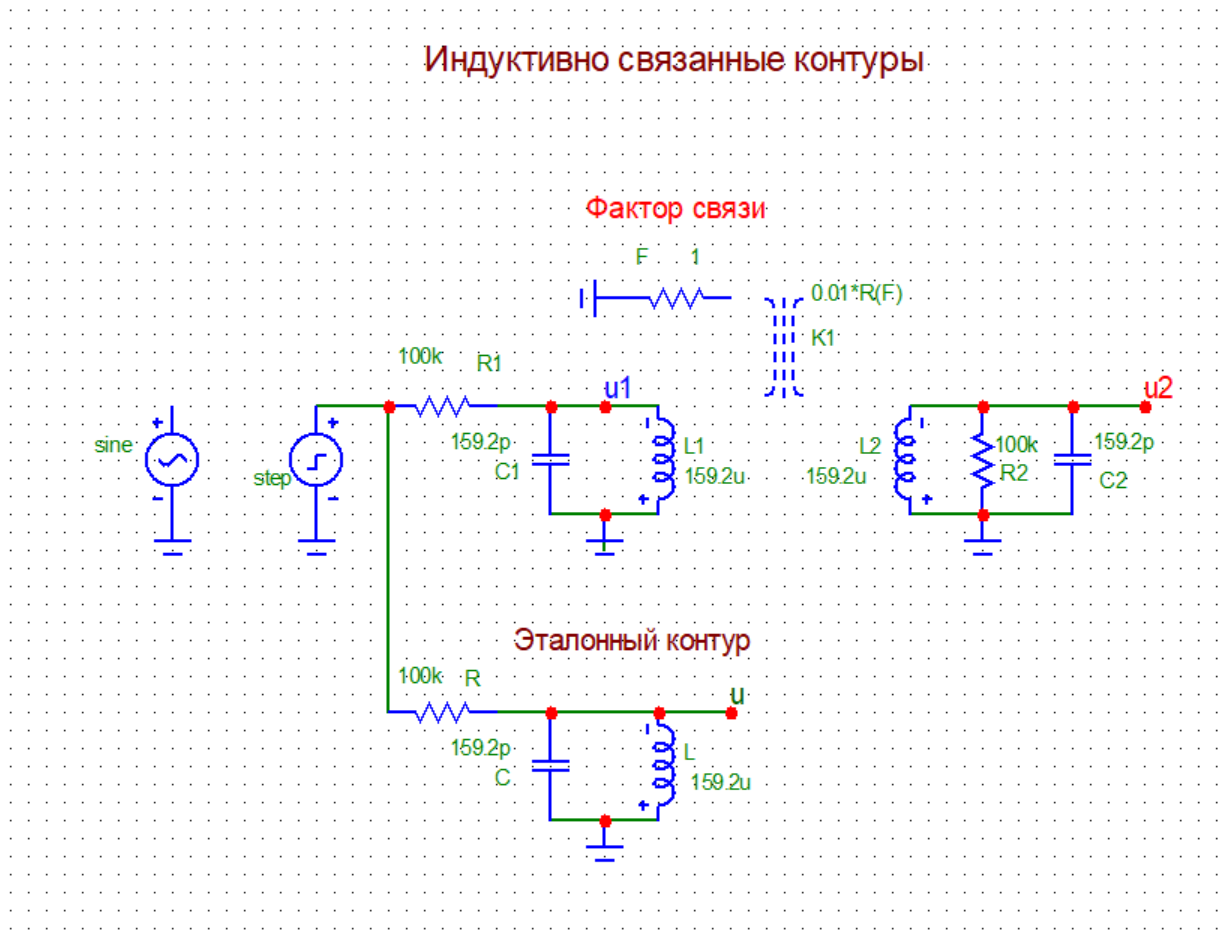
\includegraphics[scale = 0.7]{images/2LCM.png}
\label{fig:Image1}
\end{figure}

\newpage

\item Оставим только \textbf{плот 2} - просто частотные характеристики схемы. Посмотрим на поведение схемы при варьировании параметров контуров при критической связи.

\begin{figure}[h!]
%\centering
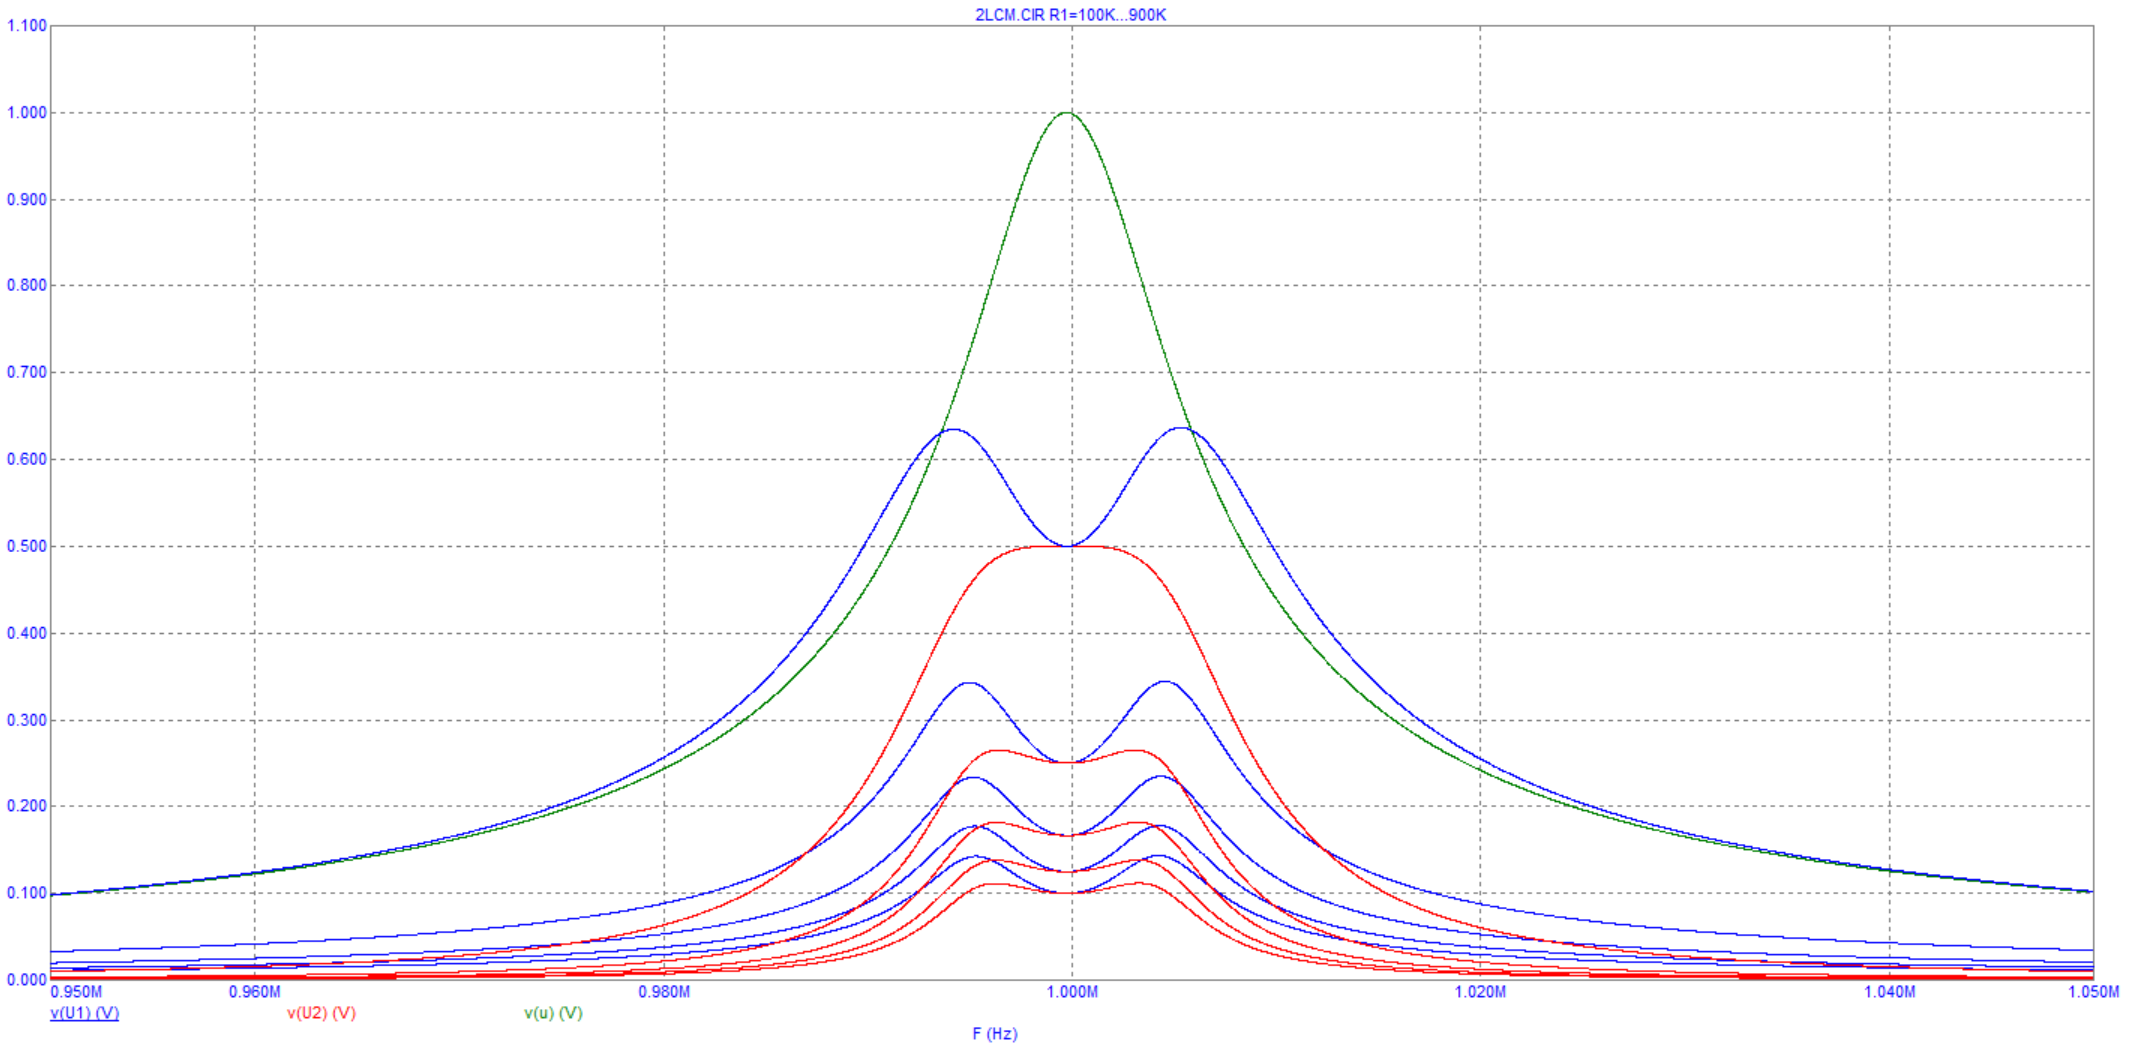
\includegraphics[scale = 0.4]{images/plot2_1.png}
\caption{$R_1 = [100k, 900k|200k], \: R_2 = 100k$}
\label{fig:Image1}
\end{figure}

\begin{figure}[h!]
\centering
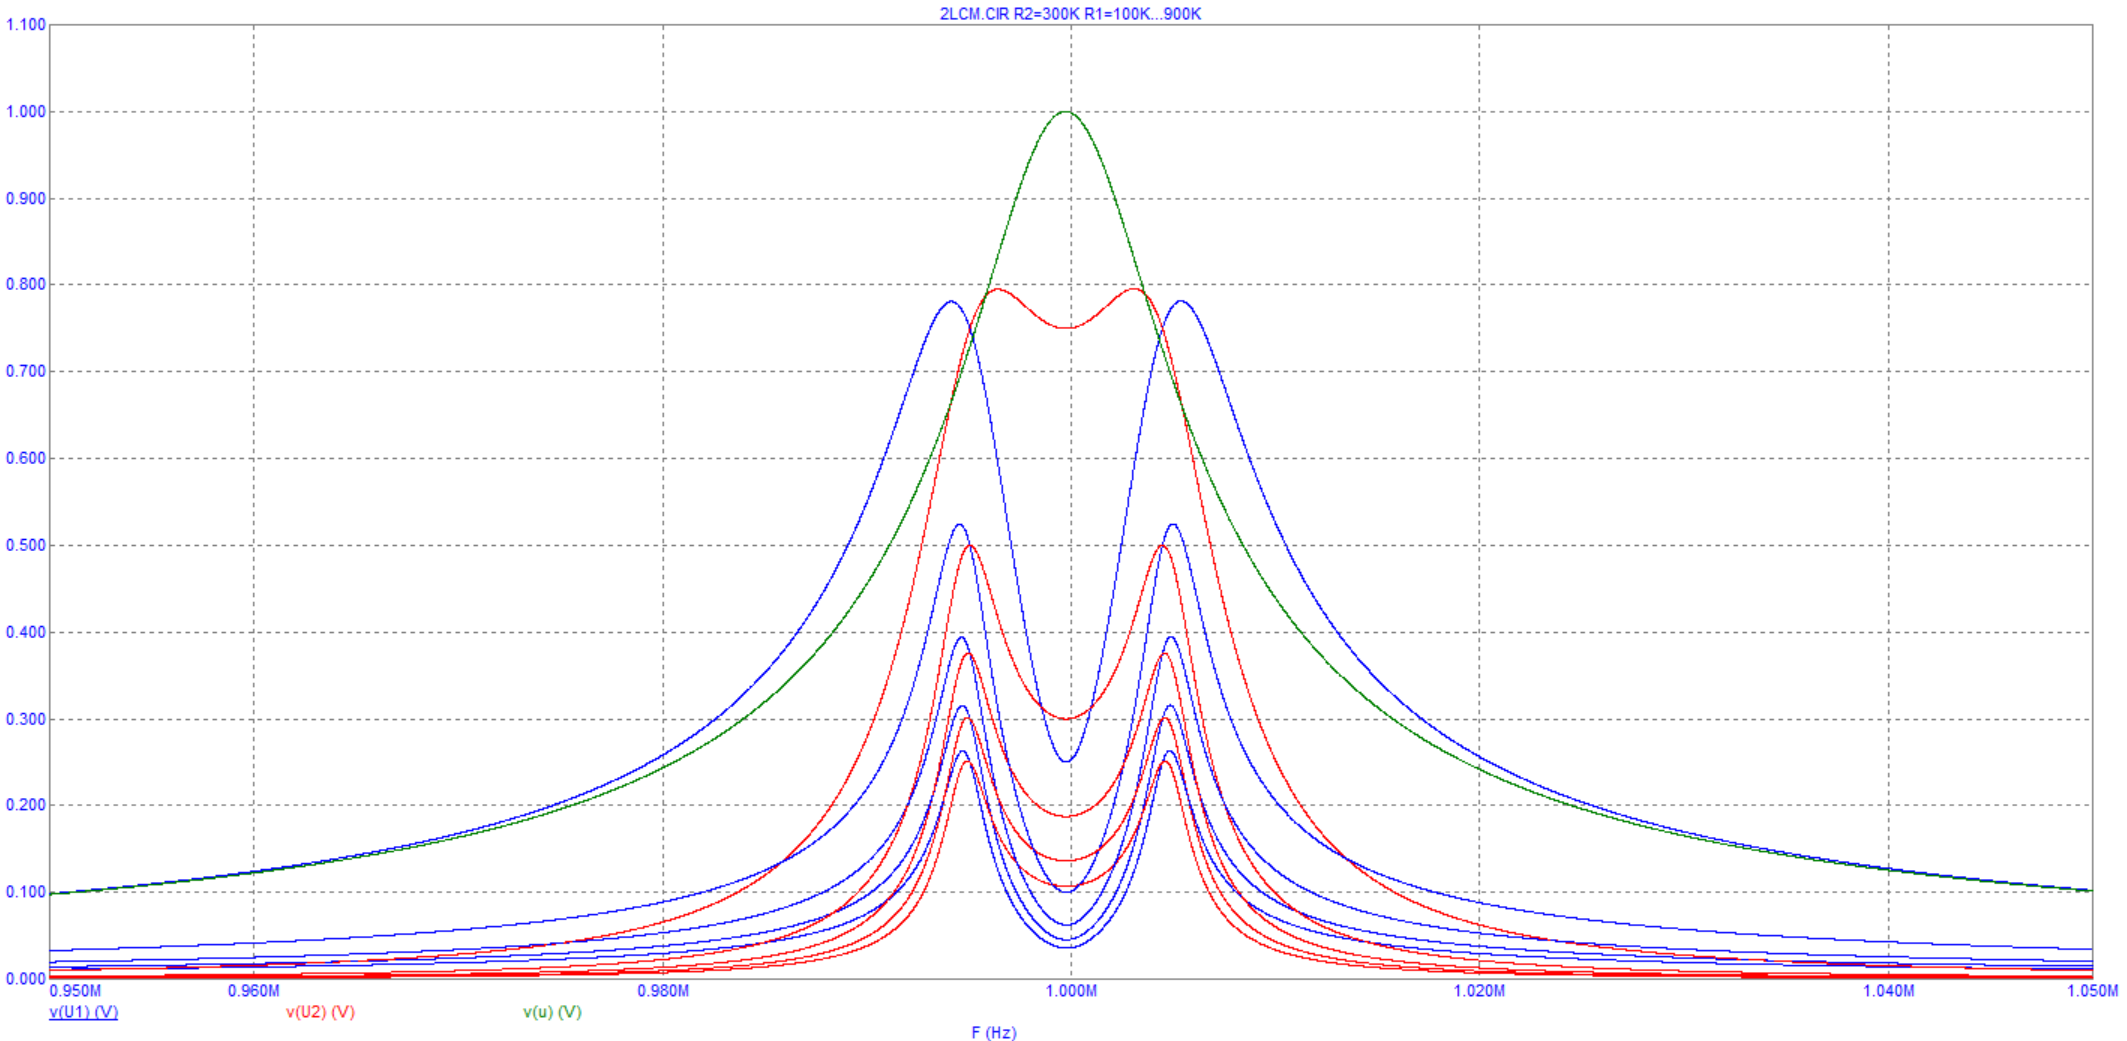
\includegraphics[scale = 0.4]{images/plot2_2.png}
\caption{$R_1 = [100k, 900k|200k], \: R_2 = 300k$}
\label{fig:Image1}
\end{figure}

\newpage

\begin{figure}[h!]
\centering
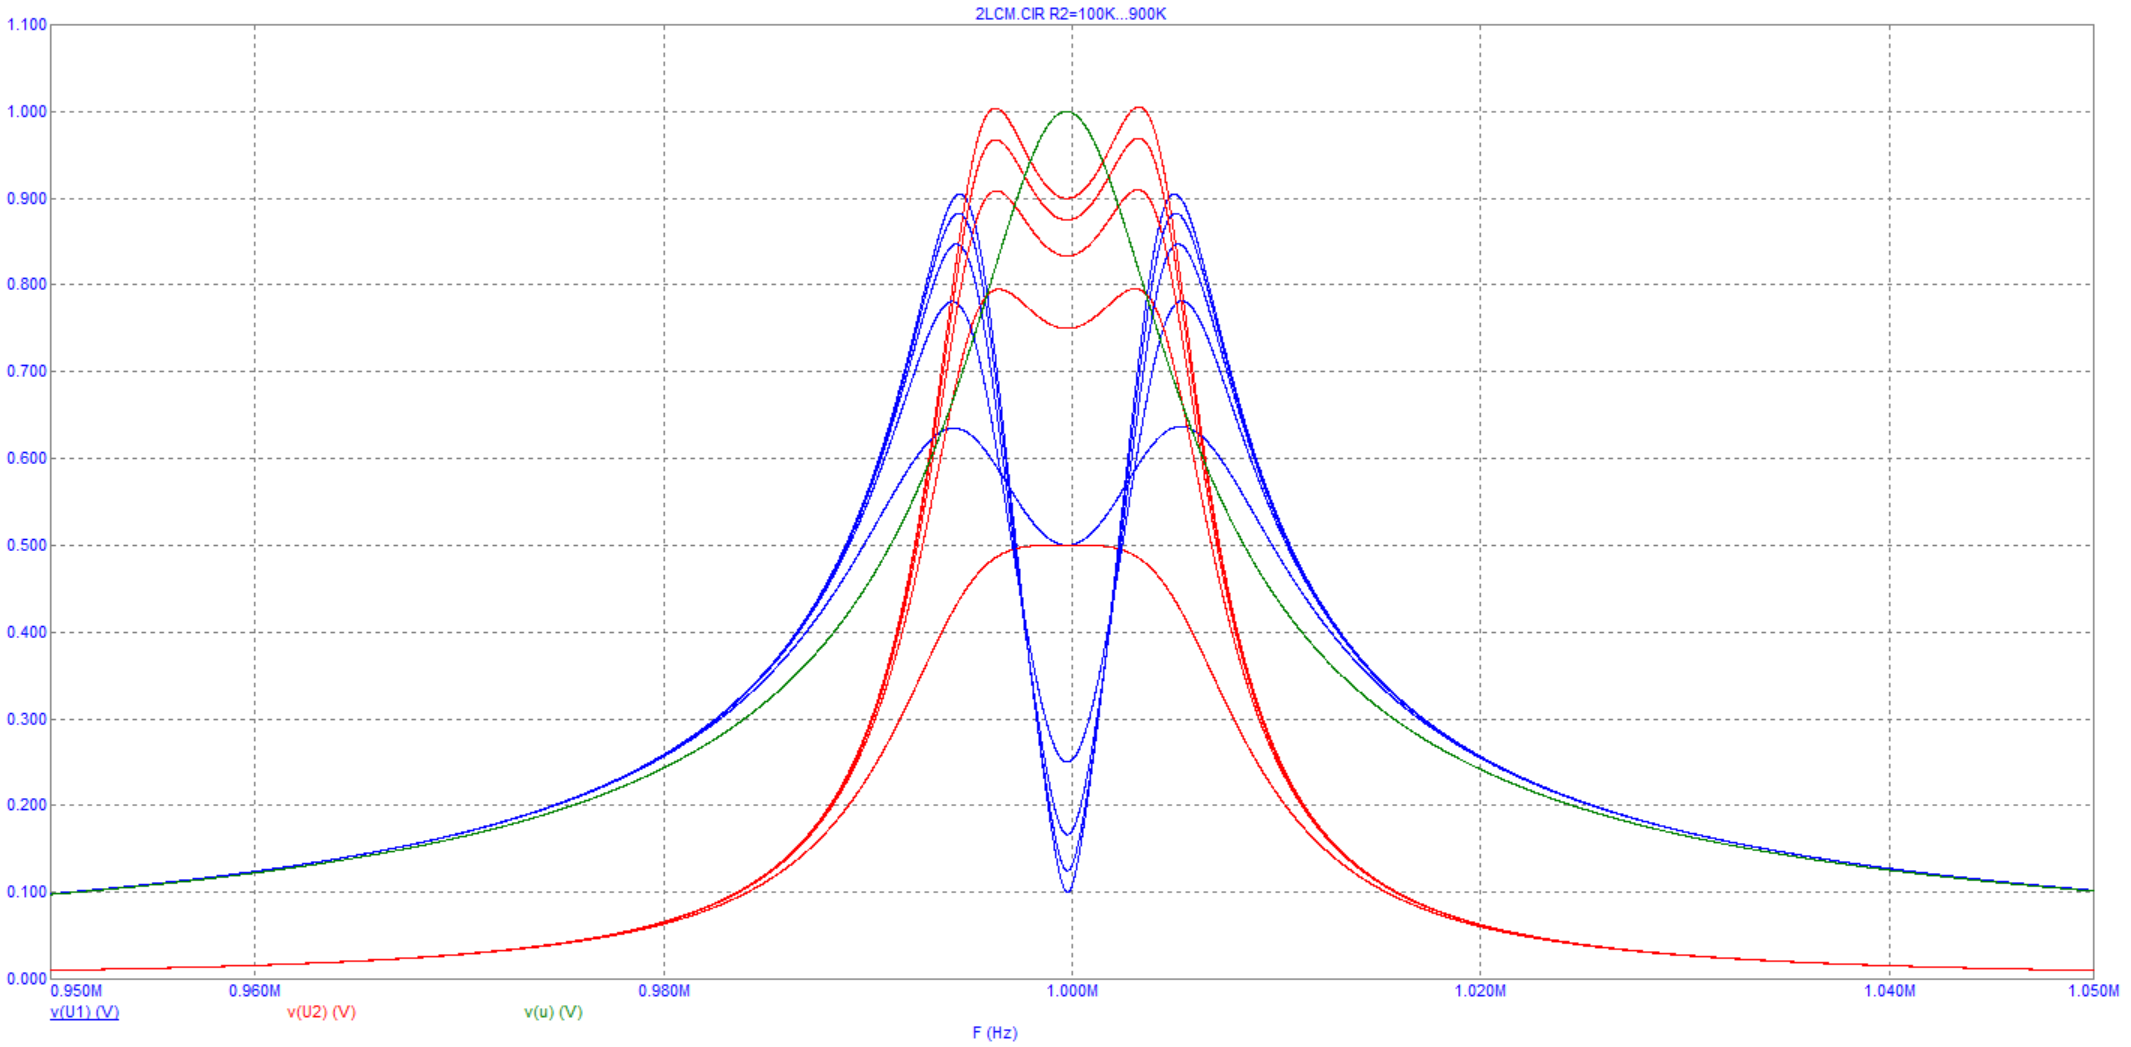
\includegraphics[scale = 0.4]{images/plot2_3.png}
\caption{$R_1 = 100k, \: R_2 = [100k, 900k|200k]$}
\label{fig:Image1}
\end{figure}

\begin{figure}[h!]
\centering
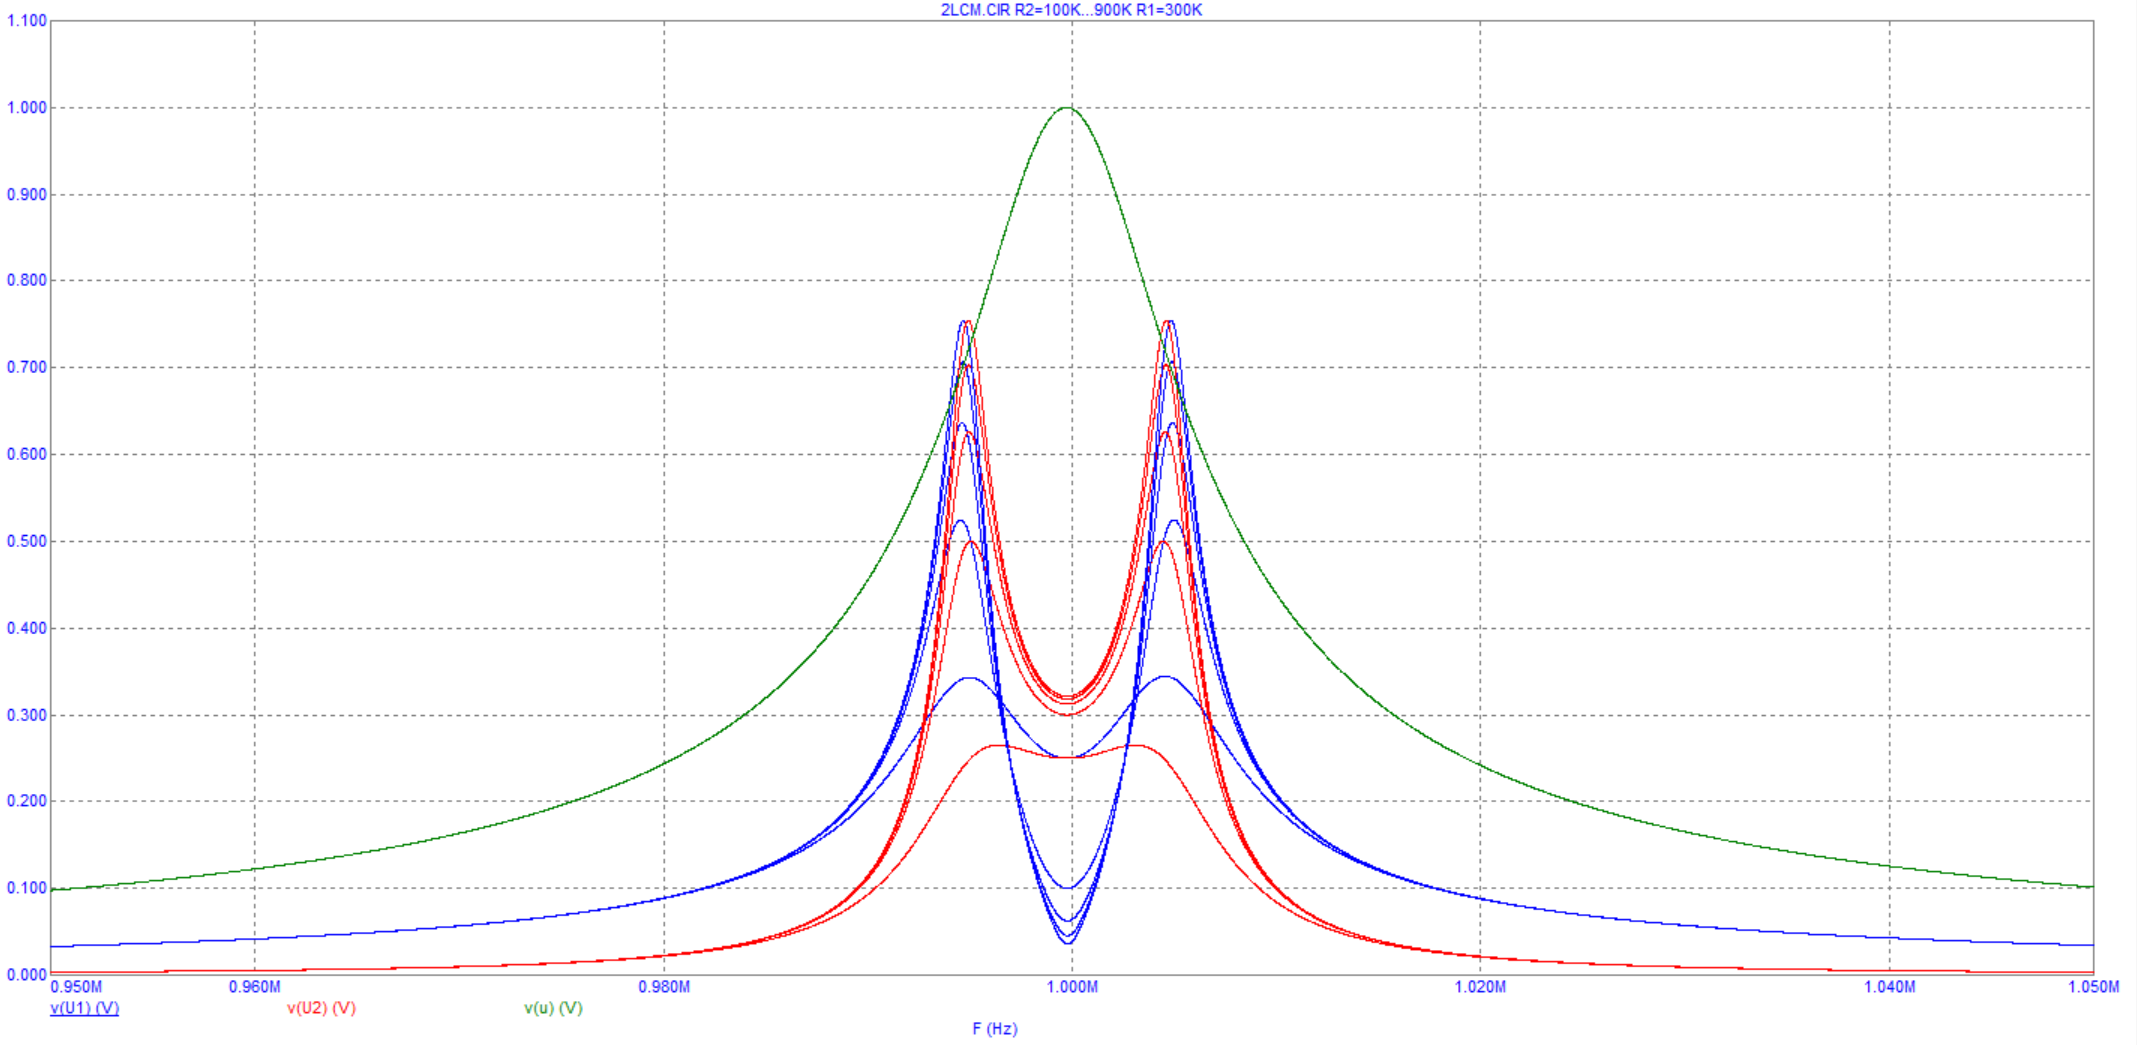
\includegraphics[scale = 0.4]{images/plot2_4.png}
\caption{$R_1 = 300k, \: R_2 = [100k, 900k|200k]$}
\label{fig:Image1}
\end{figure}

\newpage

\begin{figure}[h!]
\centering
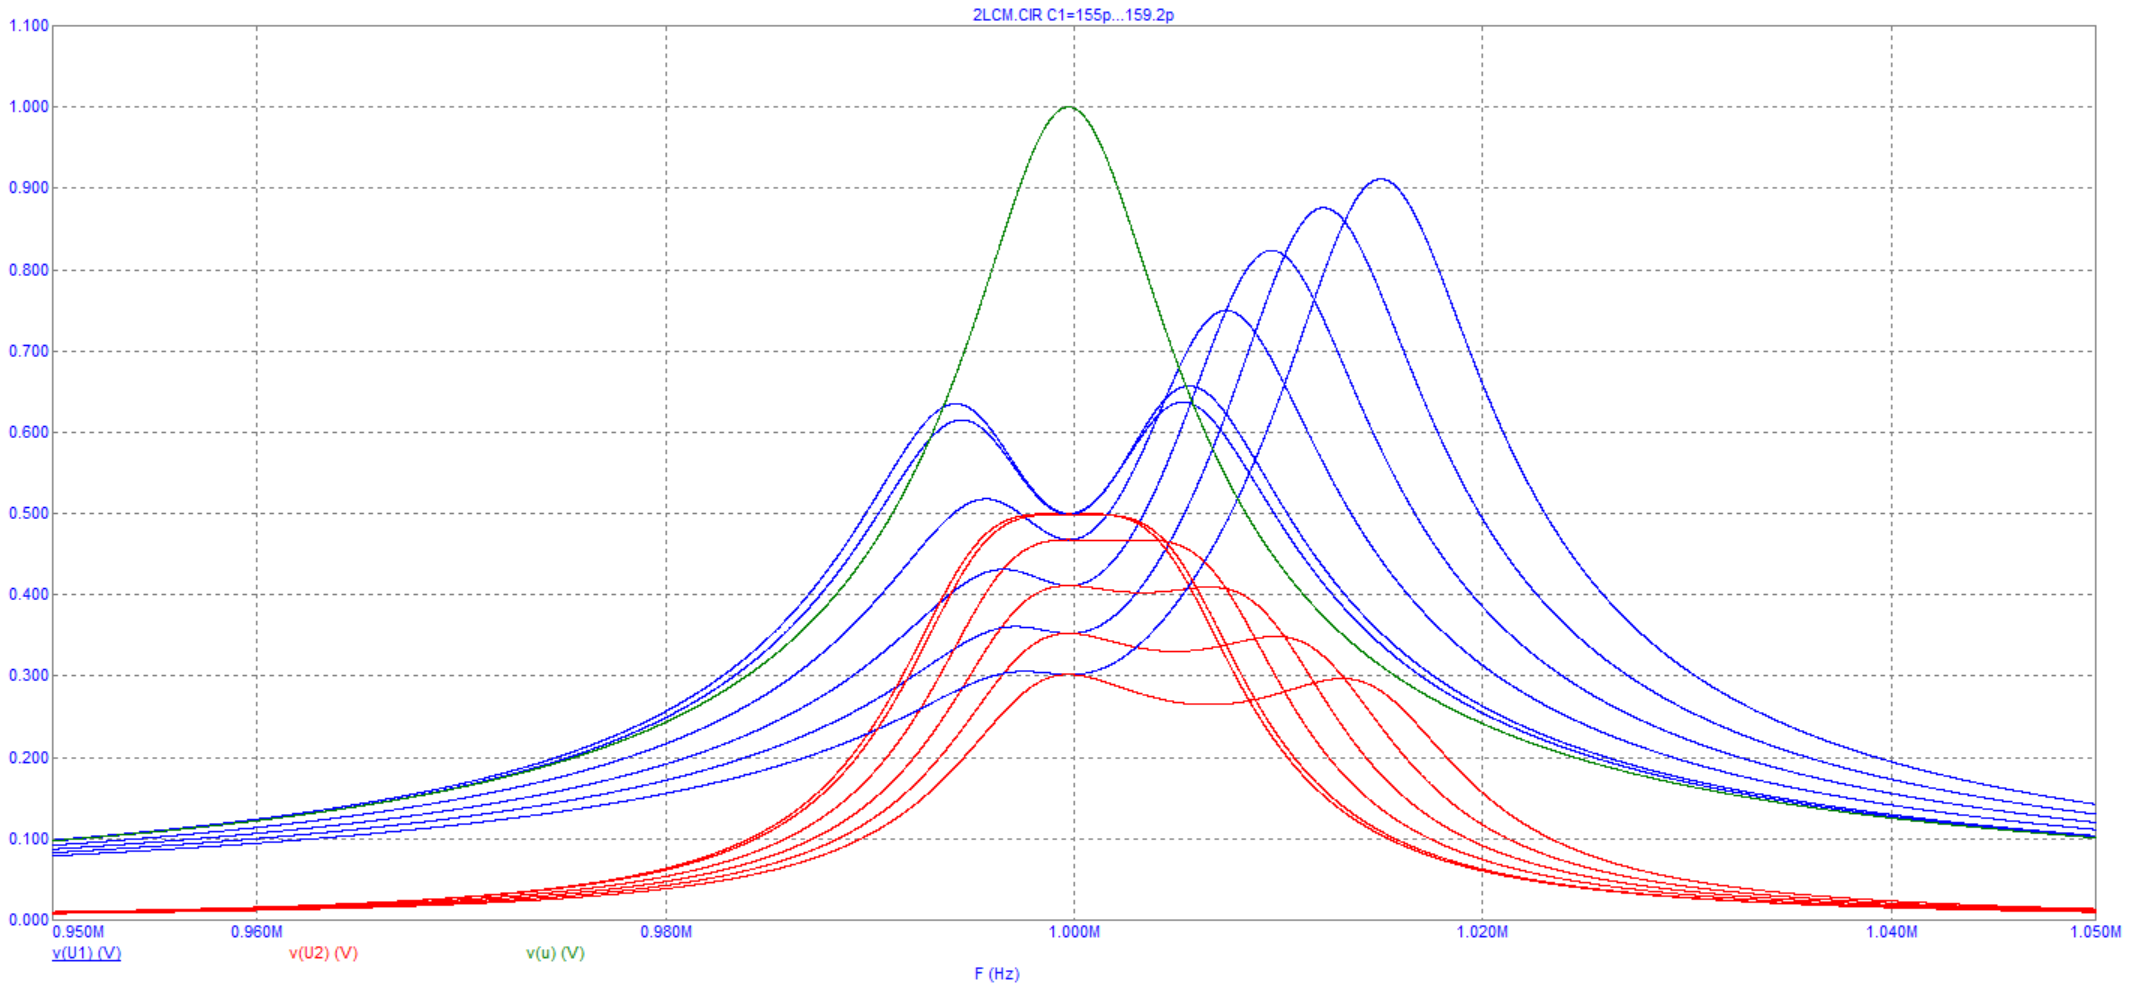
\includegraphics[scale = 0.4]{images/plot2_5.png}
\caption{$R_1 = 100k, \: R_2 = 100k, \: C_1 = [155p, 159,2p | 1p]$}
\label{fig:Image1}
\end{figure}

\begin{figure}[h!]
\centering
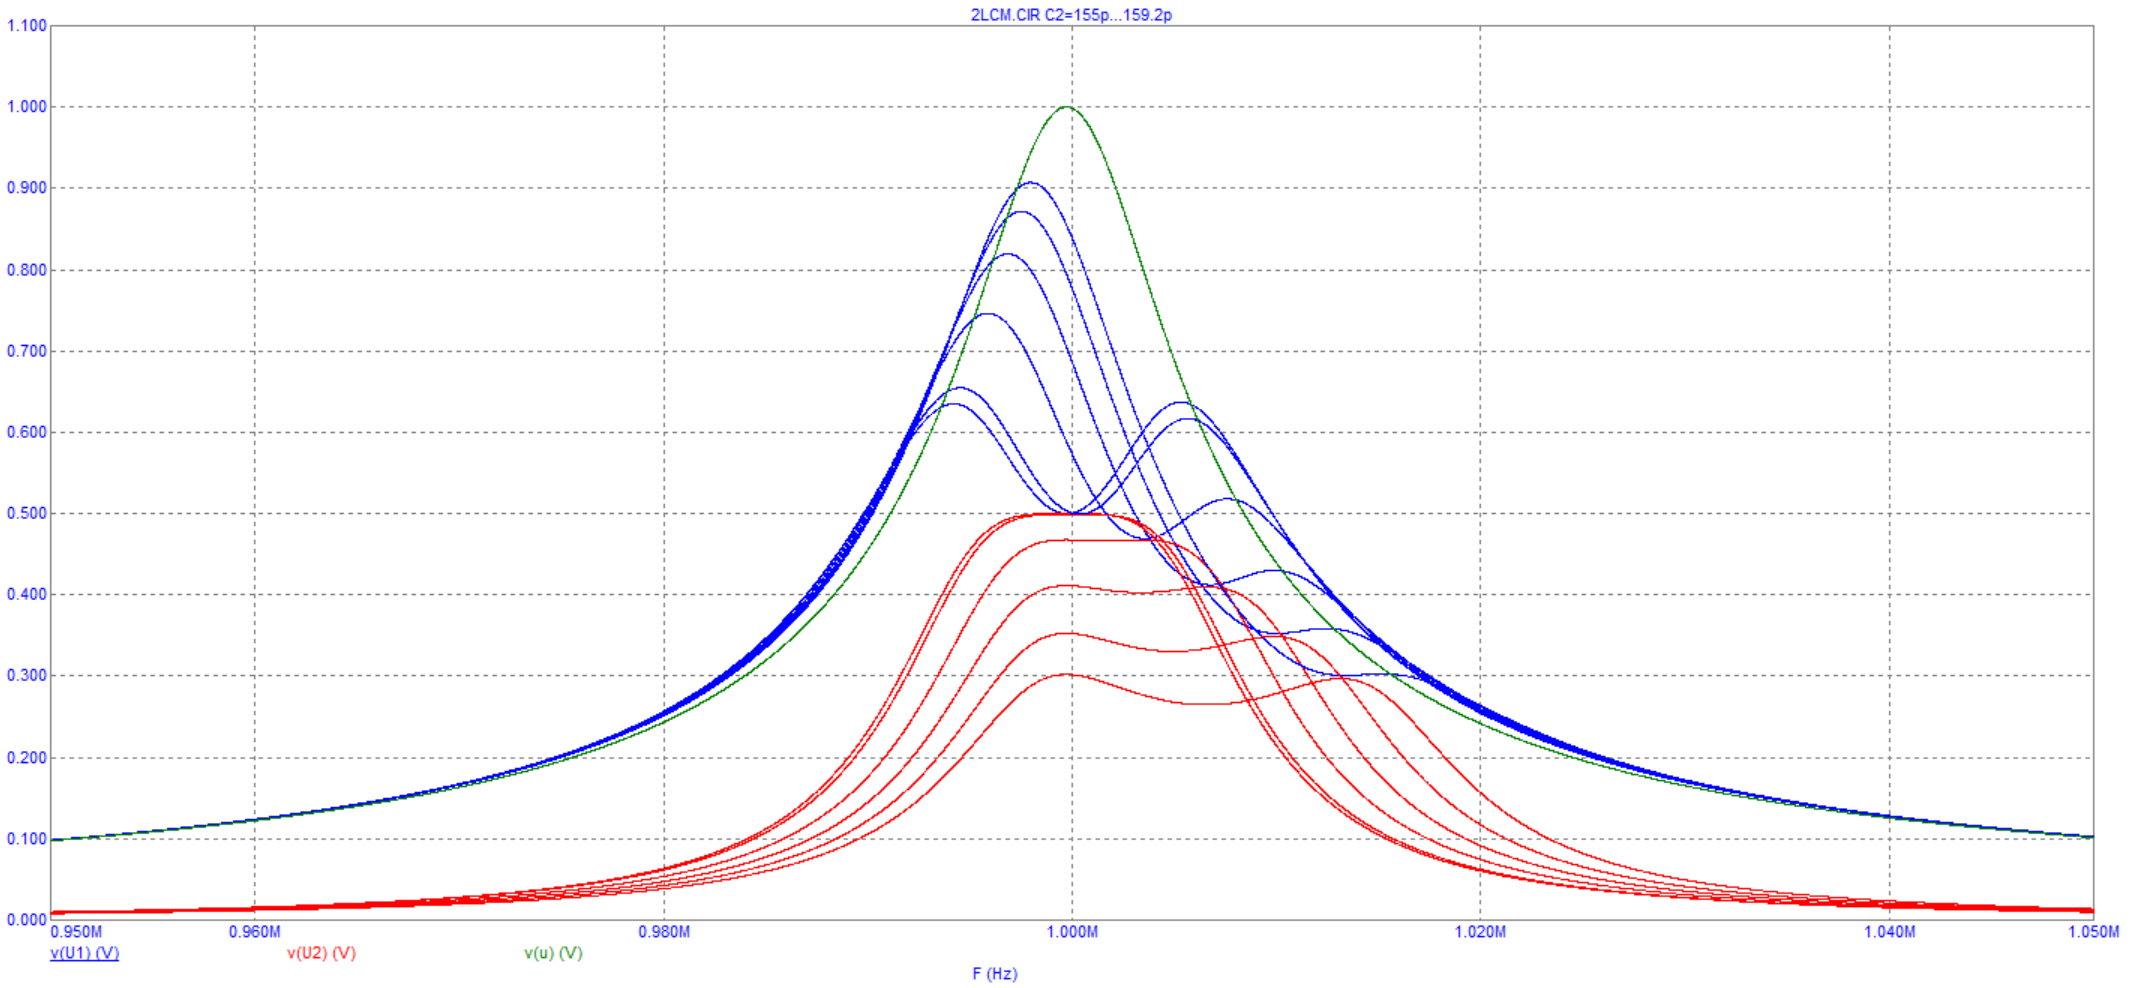
\includegraphics[scale = 0.4]{images/plot2_6.png}
\caption{$R_1 = 100k, \: R_2 = 100k, \: C_2 = [155p, 159,2p | 1p]$}
\label{fig:Image1}
\end{figure}

\newpage

\begin{figure}[h!]
\centering
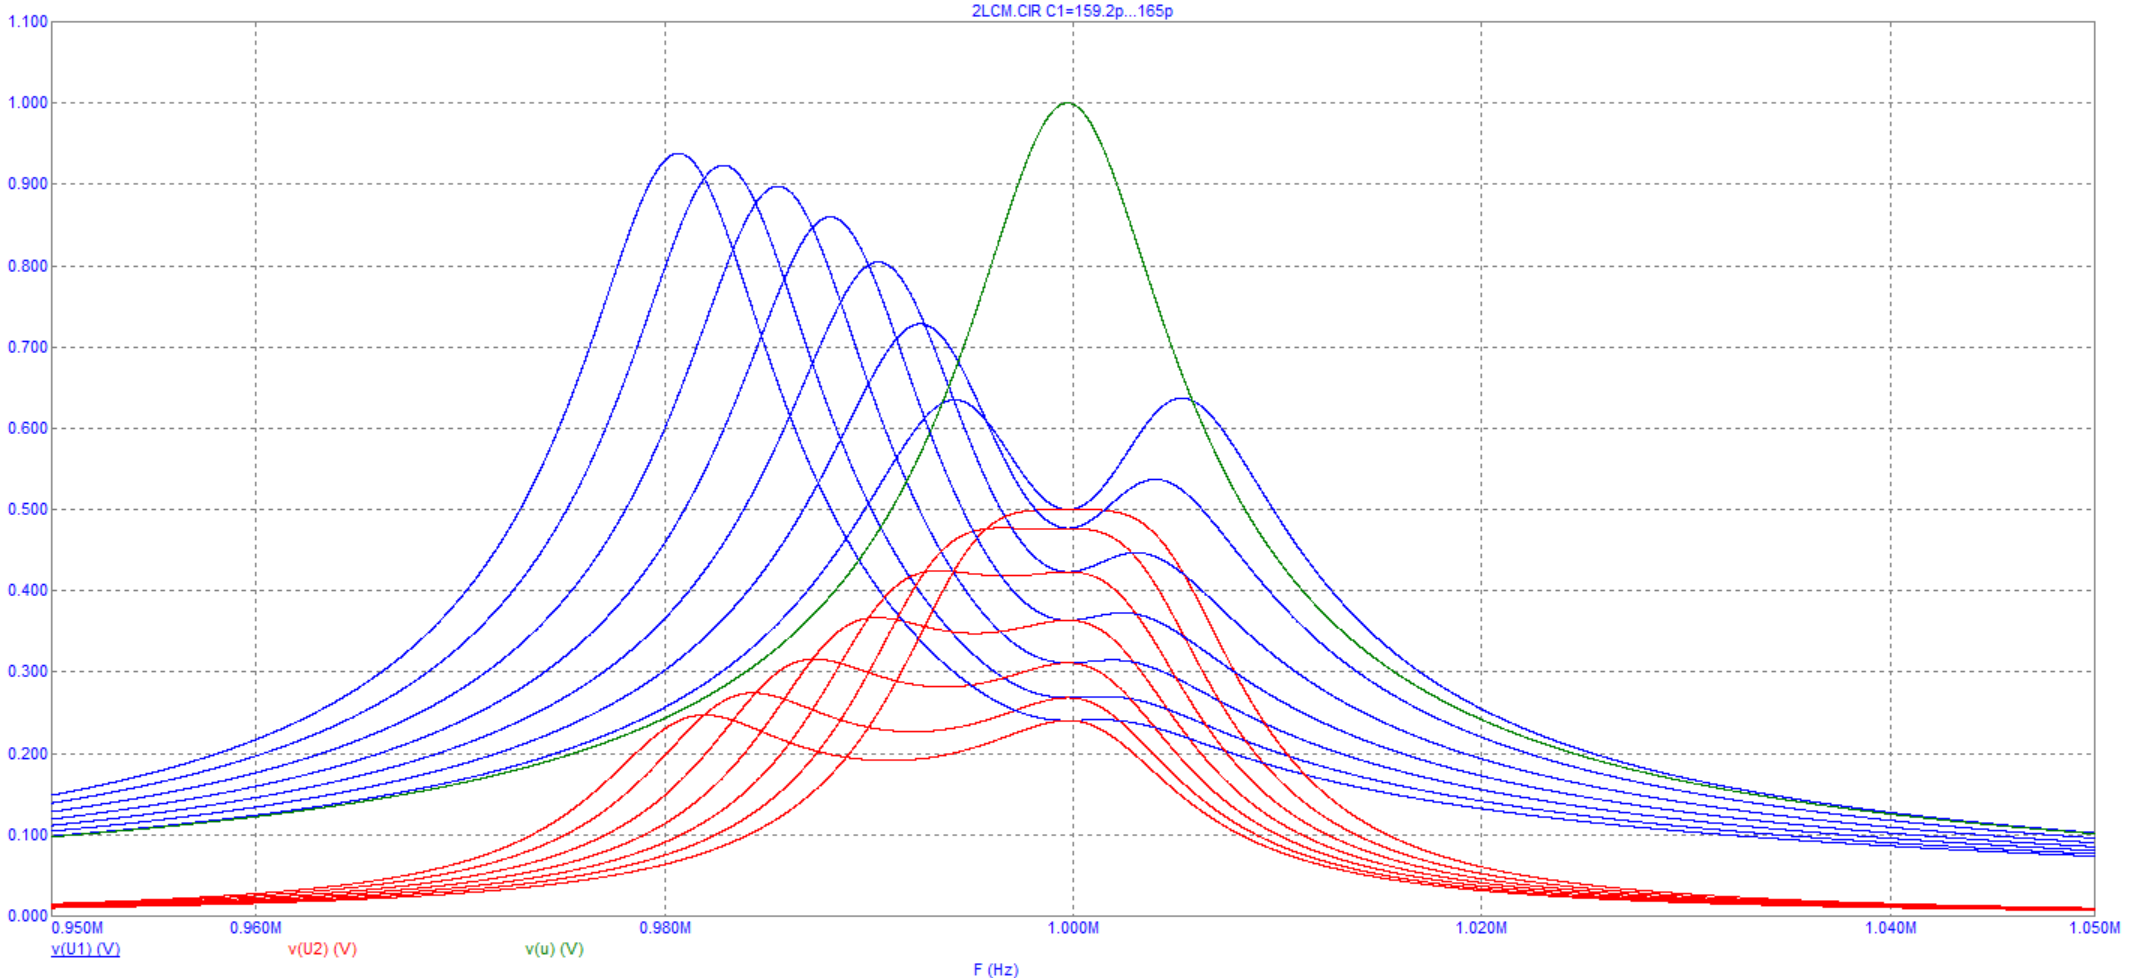
\includegraphics[scale = 0.4]{images/plot2_7.png}
\caption{$R_1 = 100k, \: R_2 = 100k, \: C_1 = [159,2p, 165p | 1p]$}
\label{fig:Image1}
\end{figure}

\begin{figure}[h!]
\centering
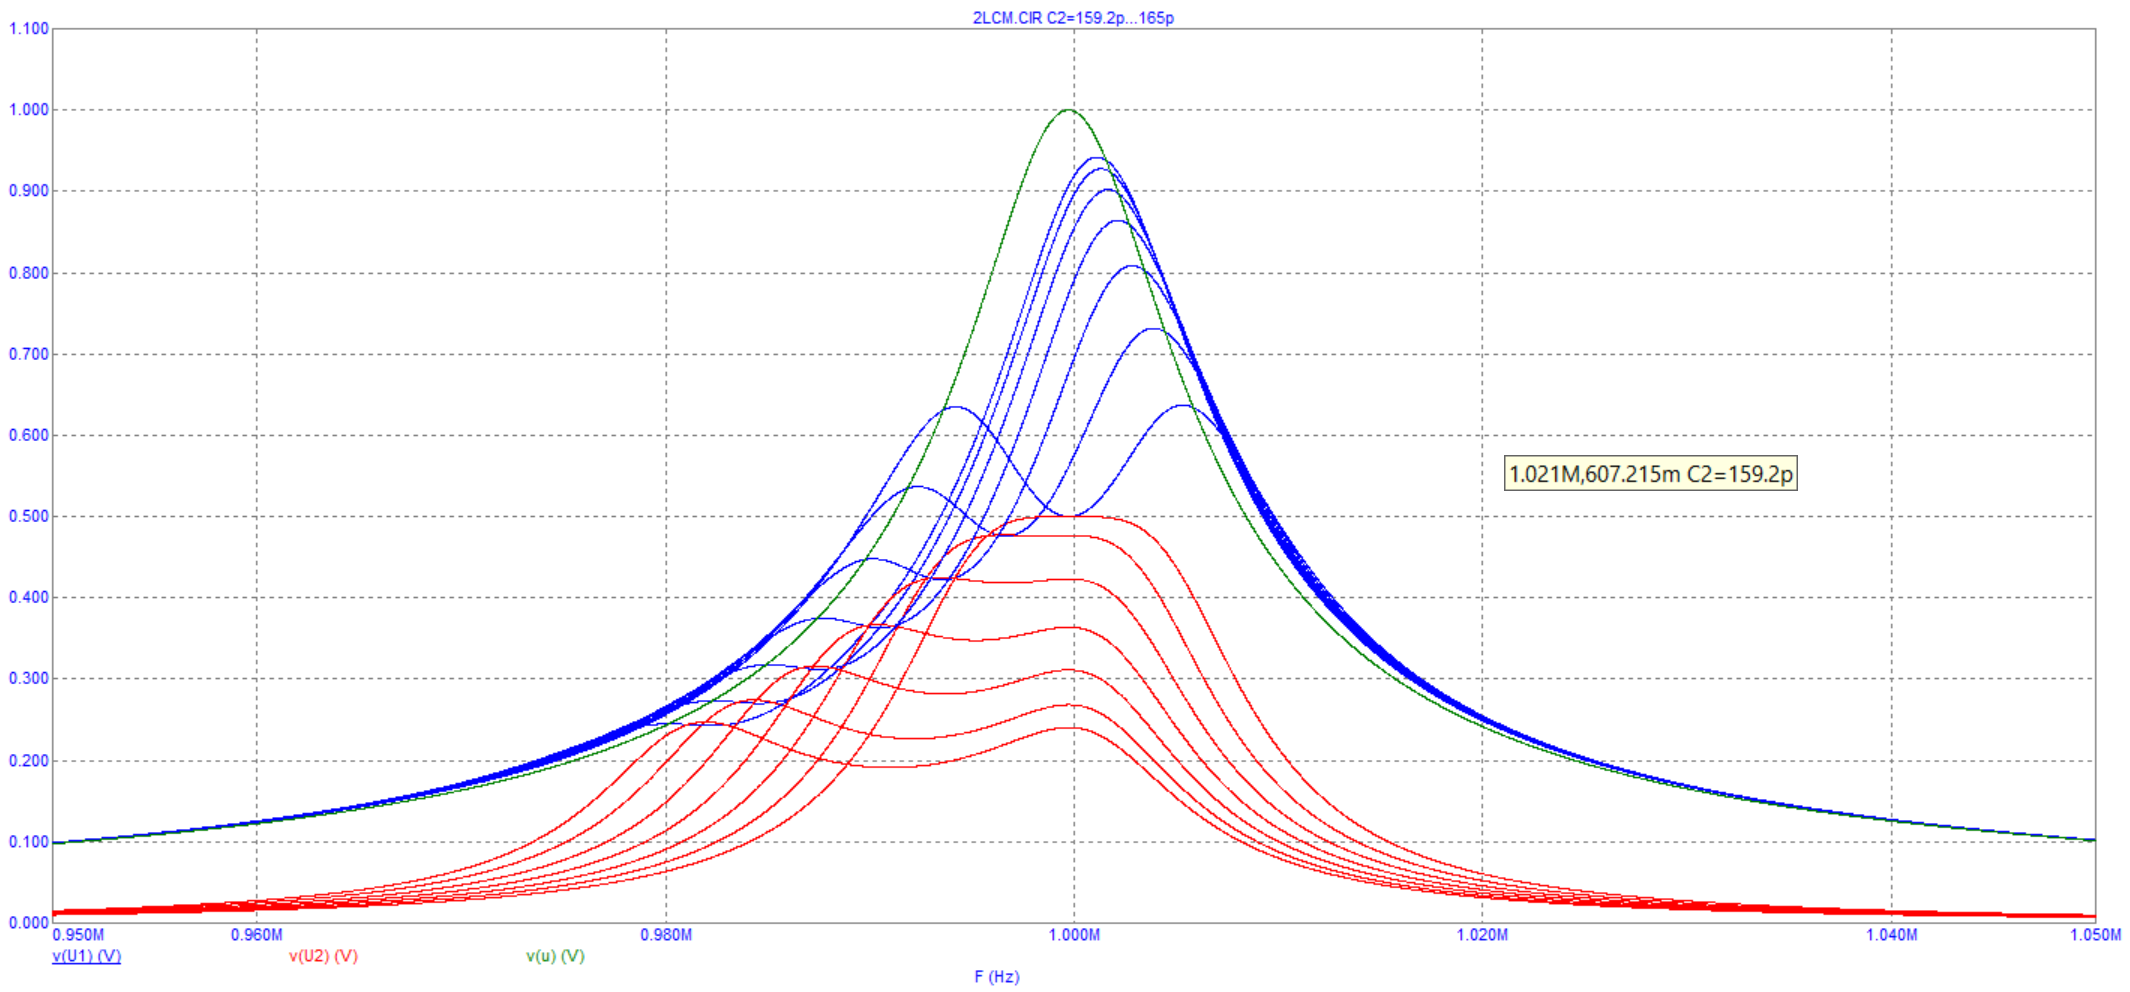
\includegraphics[scale = 0.4]{images/plot2_8.png}
\caption{$R_1 = 100k, \: R_2 = 100k, \: C_2 = [159,2p, 165p | 1p]$}
\label{fig:Image1}
\end{figure}

\newpage

\item Изучим поведение резонансных кривых и фазовых характеристик при $F = [0.2, 1 | 0.2]$ и $F = [1, 5 | 1]$. 

\begin{figure}[h!]
\centering
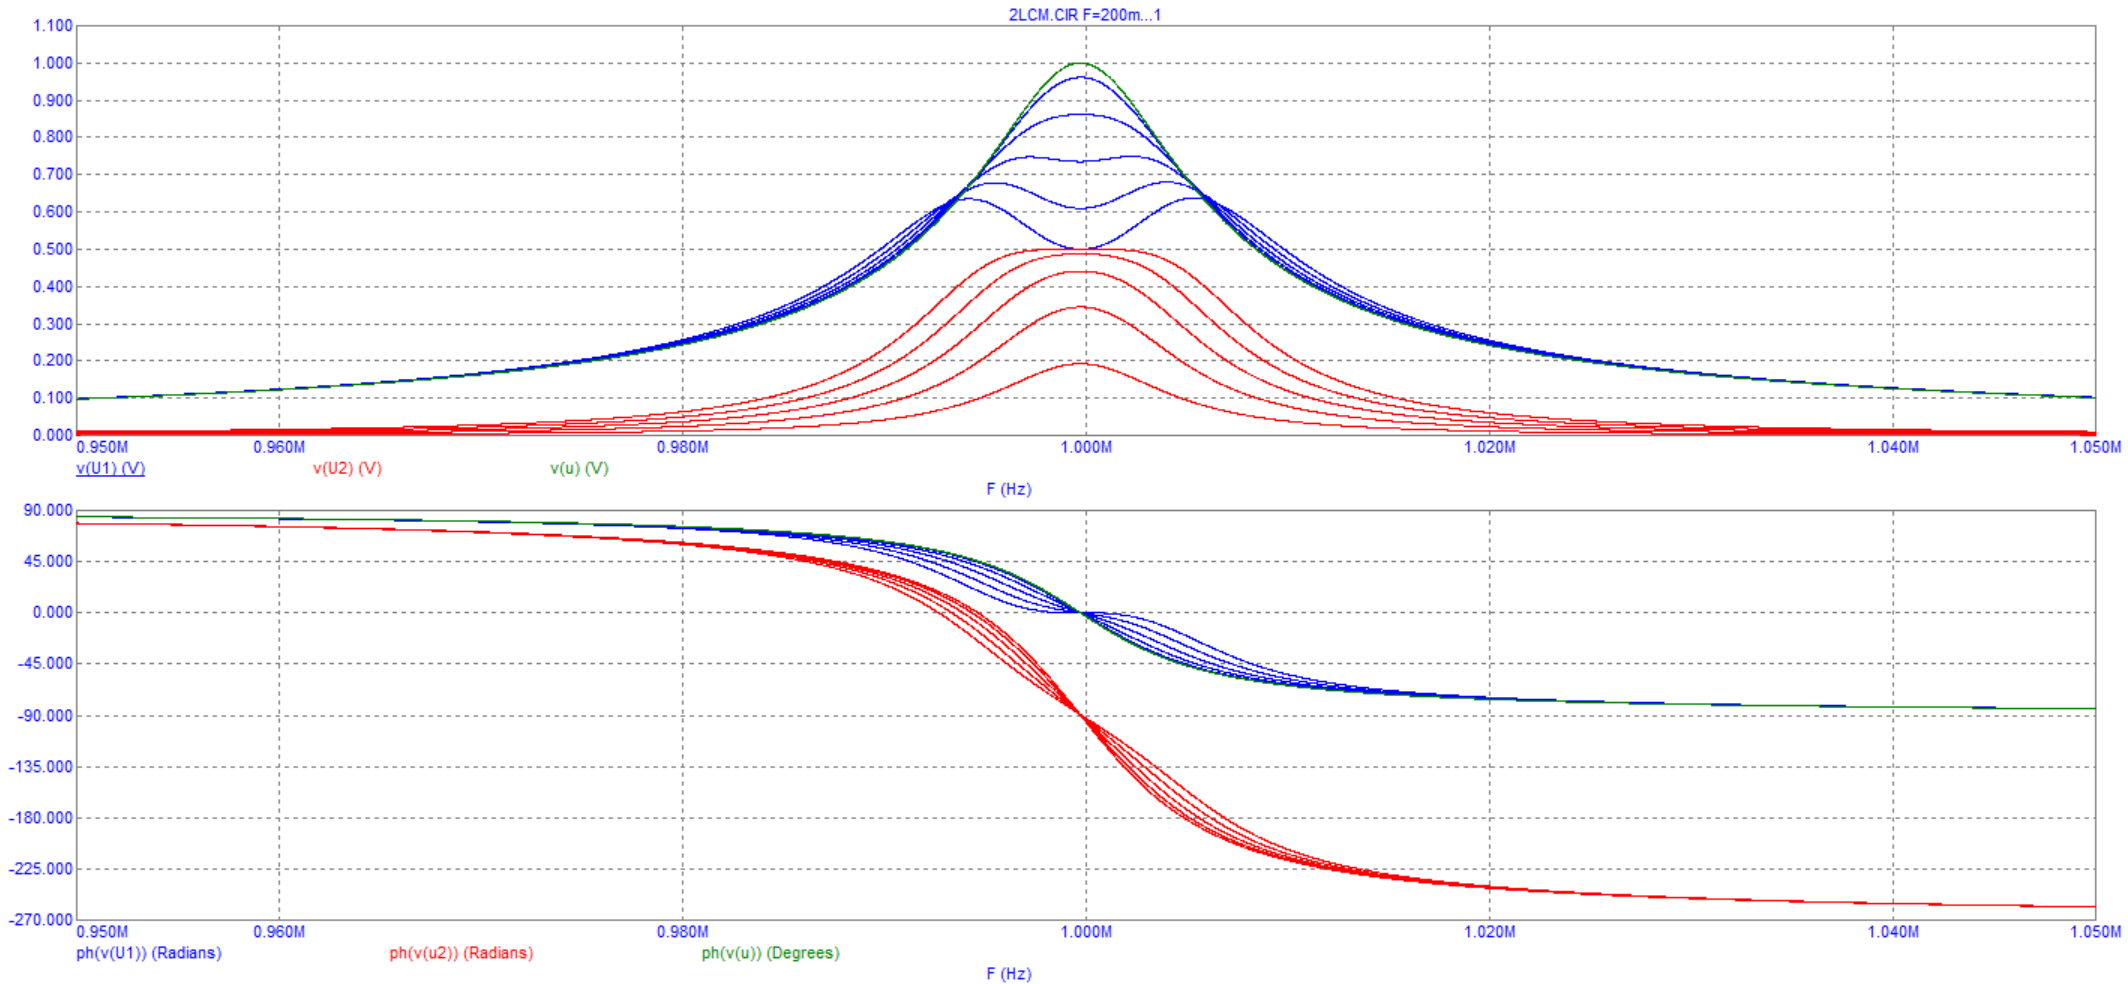
\includegraphics[scale = 0.4]{images/plot3_1.png}
\caption{$F = [0.2, 1 | 0.2]$}
\label{fig:Image1}
\end{figure}

\begin{figure}[h!]
\centering
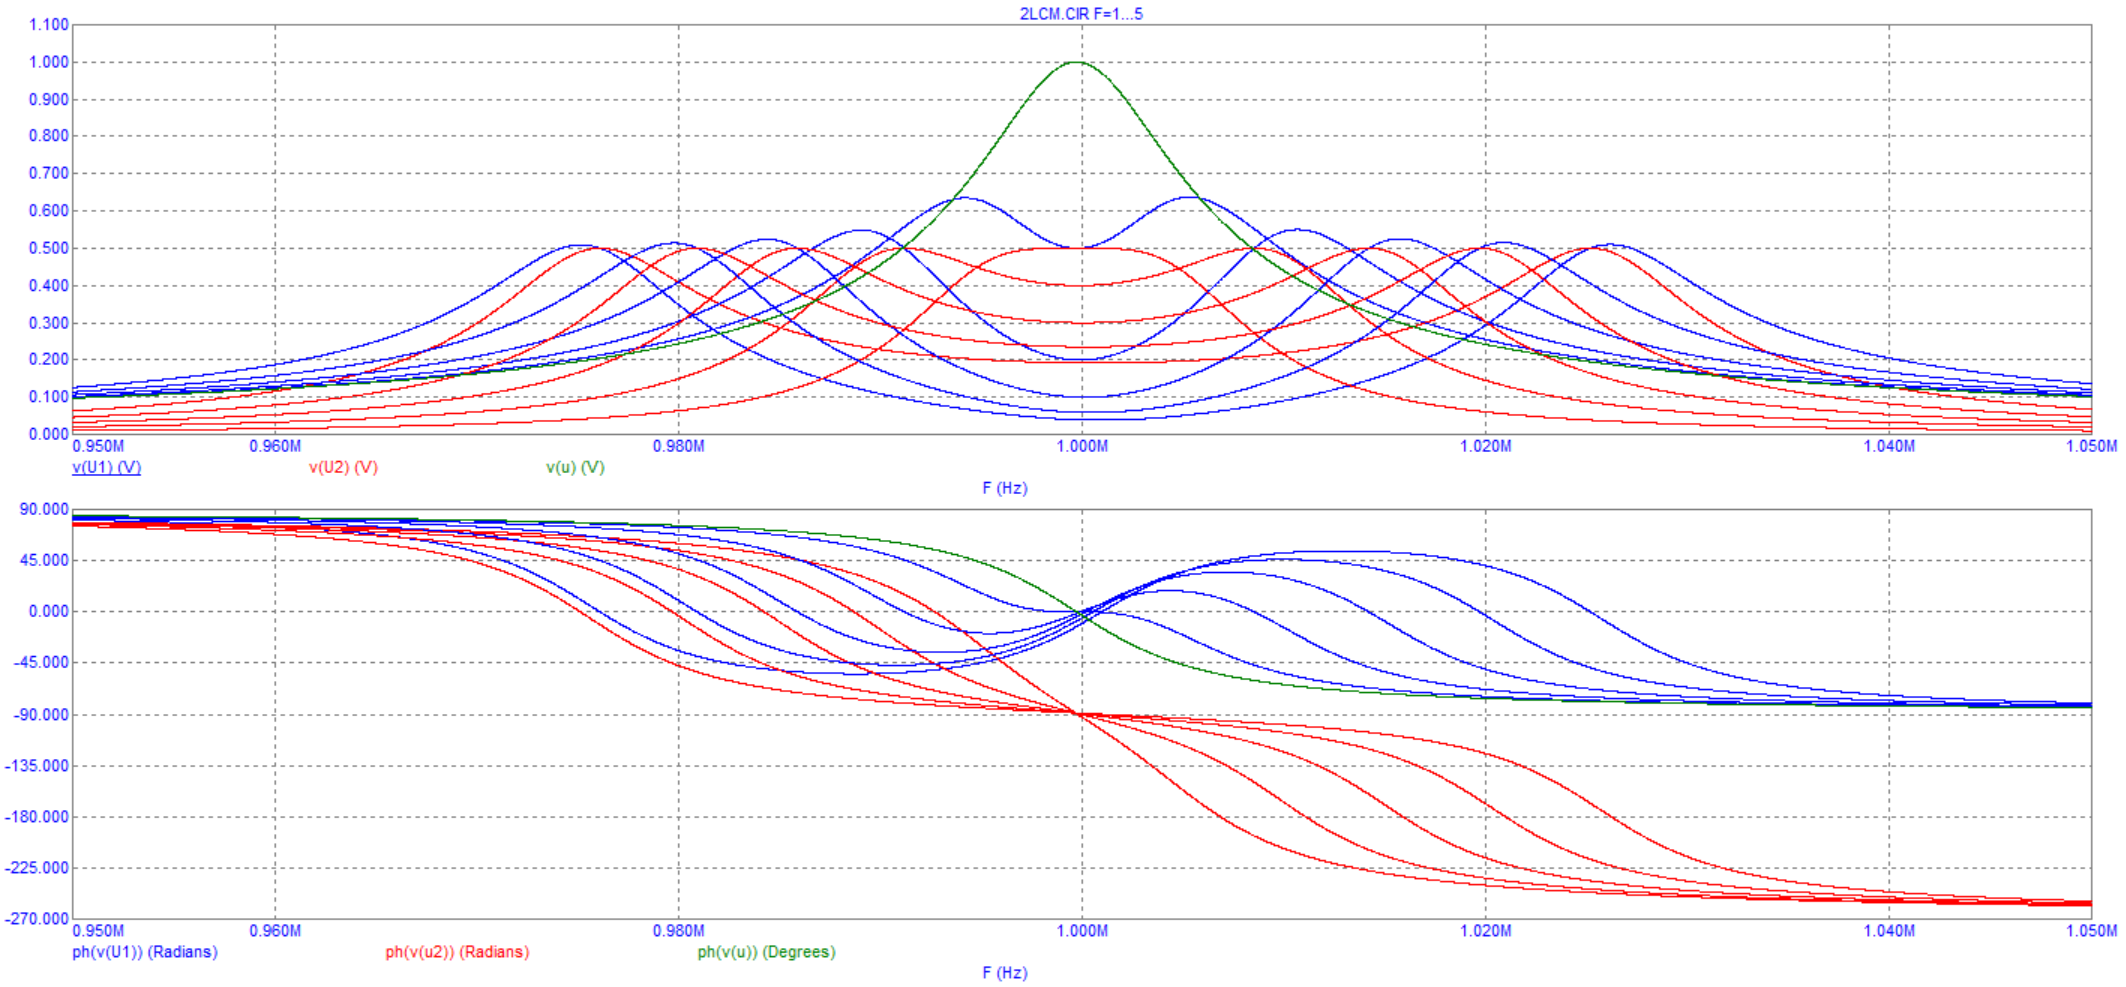
\includegraphics[scale = 0.4]{images/plot3_2.png}
\caption{$F = [1, 5 | 1]$}
\label{fig:Image1}
\end{figure}

Измерим границы диапазонов изменения фаз на первом и втором контурах:

На первом контуре - от  $-84.14^{\circ}$ до $84.43^{\circ}$, на втором контуре - от $-258.36^{\circ}$ до $-78.34^{\circ}$,

А также разность фаз между напряжениями на контурах на частоте $f_0:$ $89.27^{\circ}$.

Измерив уровни $u_1(f_0)$, $u_2(f_0)$ при $F = 0.5; 1; 2,$ проверим формулы:

\begin{equation}
u_1(f_0) = \frac{1}{1 + F^2}, \: u_2(f_0) = \frac{F}{1 + F^2}
\end{equation}

\begin{center}
\begin{tabular}{|c|c|c|c|}
\hline 
F & 1 & 0.5 & 2 \\ 
\hline 
$u_1(f_0)_{\text{эксп}}$ & 0.5 & 0.8 & 0.2 \\ 
\hline 
$u_1(f_0)_{\text{теор}}$ & 0.5 & 0.8 & 0.2 \\ 
\hline 
$u_2(f_0)_{\text{эксп}}$ & 0.5 & 0.4 & 0.2 \\ 
\hline 
$u_2(f_0)_{\text{теор}}$ & 0.5 & 0.4 & 0.4 \\ 
\hline 
\end{tabular}
\end{center}

Формула (1) выполняется.

\newpage

\item Измерим значения $F$, при которых возникает: a) провал на первом контуре: $F \approx 0.55$, b) провал на втором контуре: $F > 1$, с) подъем на фазовой характеристике первого контура: $F > 1$.

Измерив частоты пересечения нуля фазовой характеристикой $u_1$ при $F = 5$ ($\nu = 976.121k, 1.001M, 1.025M$) и при $F = 10$ ($\nu = 953.48k, 1.05M, 1.03M$), проверим приближённые ($f_0 \pm FF_0$) и уточнённые ($f_0\sqrt{1 \pm \frac{F}{Q}}$).

\begin{figure}[h!]
\centering
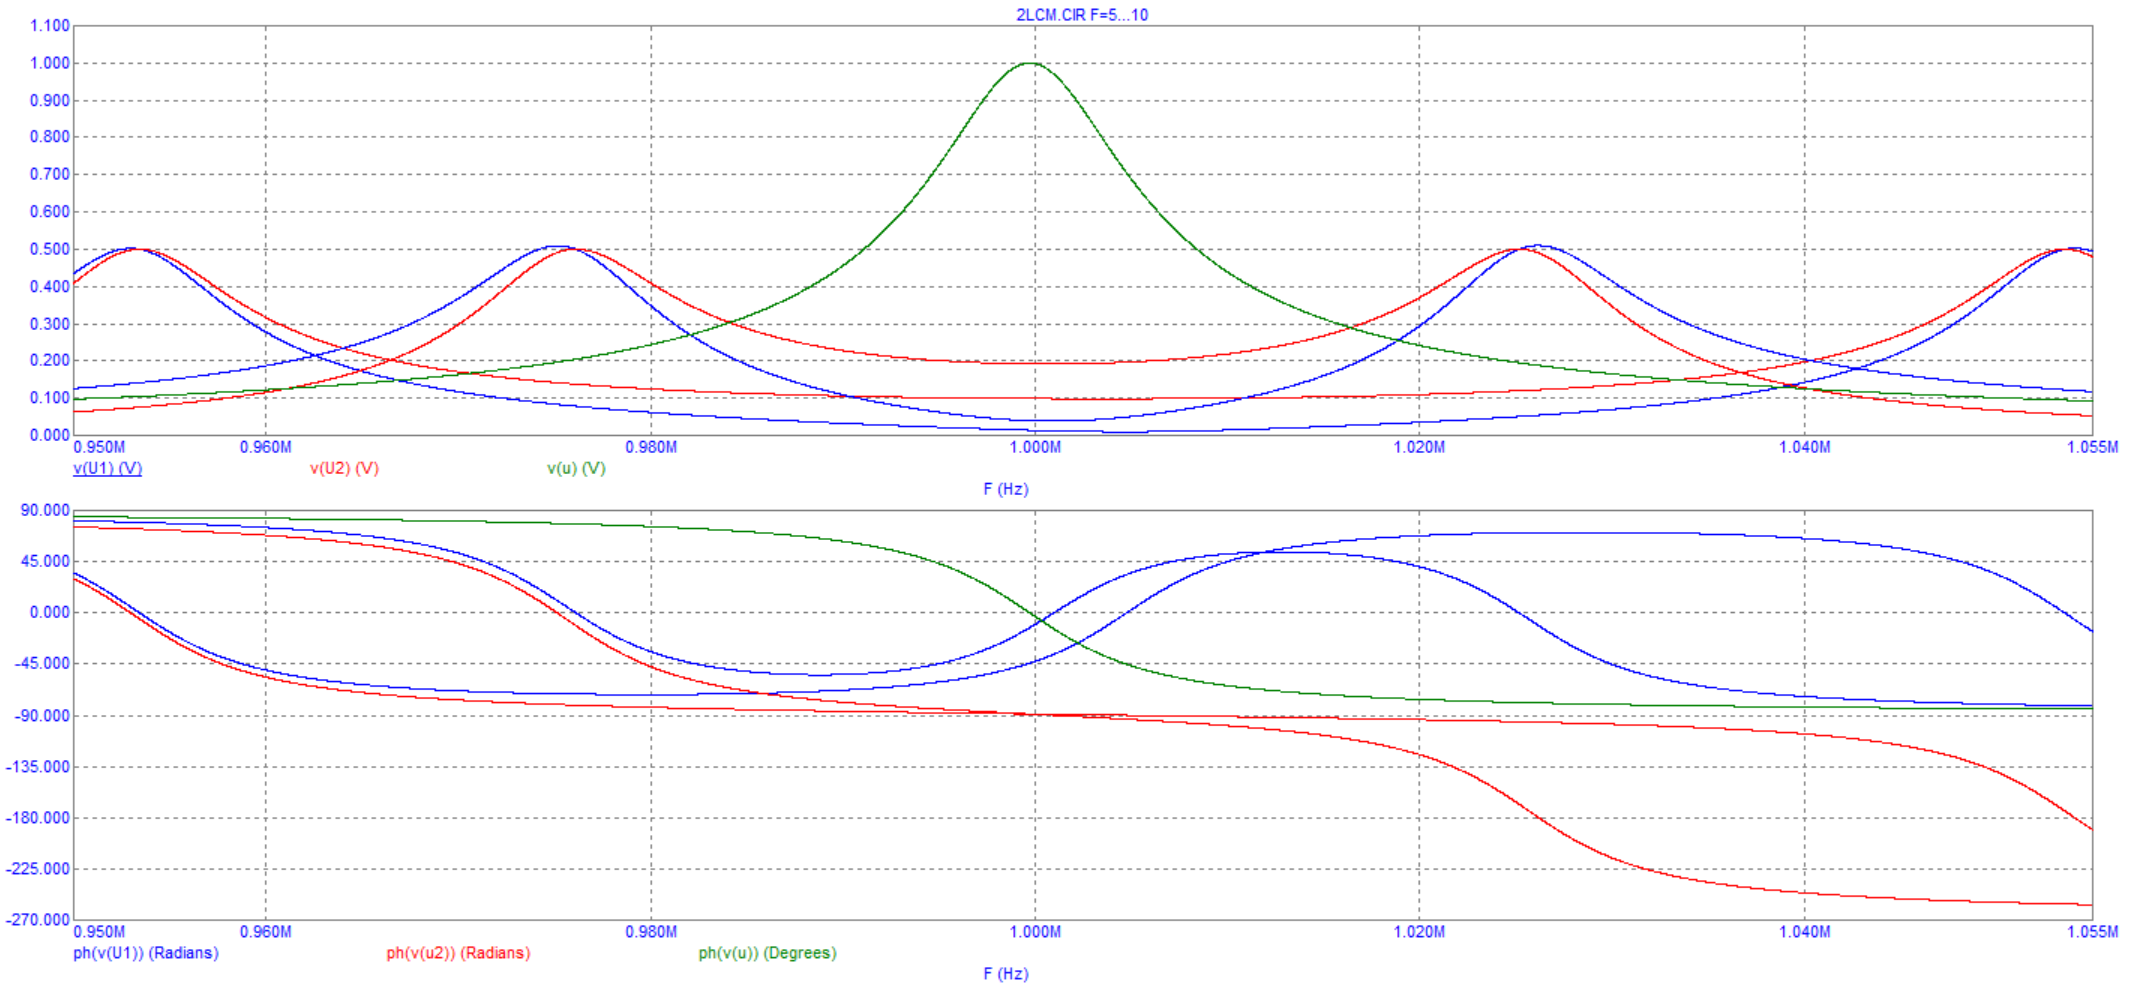
\includegraphics[scale = 0.4]{images/plot4_1.png}
\caption{$F = [5, 10 | 5]$}
\label{fig:Image1}
\end{figure}

\newpage

\item Оставим только плот 1. При критической связи измерим ширину полосы по уровню
-3dB эталонного контура ($\bigtriangleup f = 10.24k$) и ширину полосы по уровню -9dB резонансной кривой на втором контуре ($\bigtriangleup f = 14.279k$). Убедимся, что их отношение составляет $\sqrt{2}$.

\begin{figure}[h!]
\centering
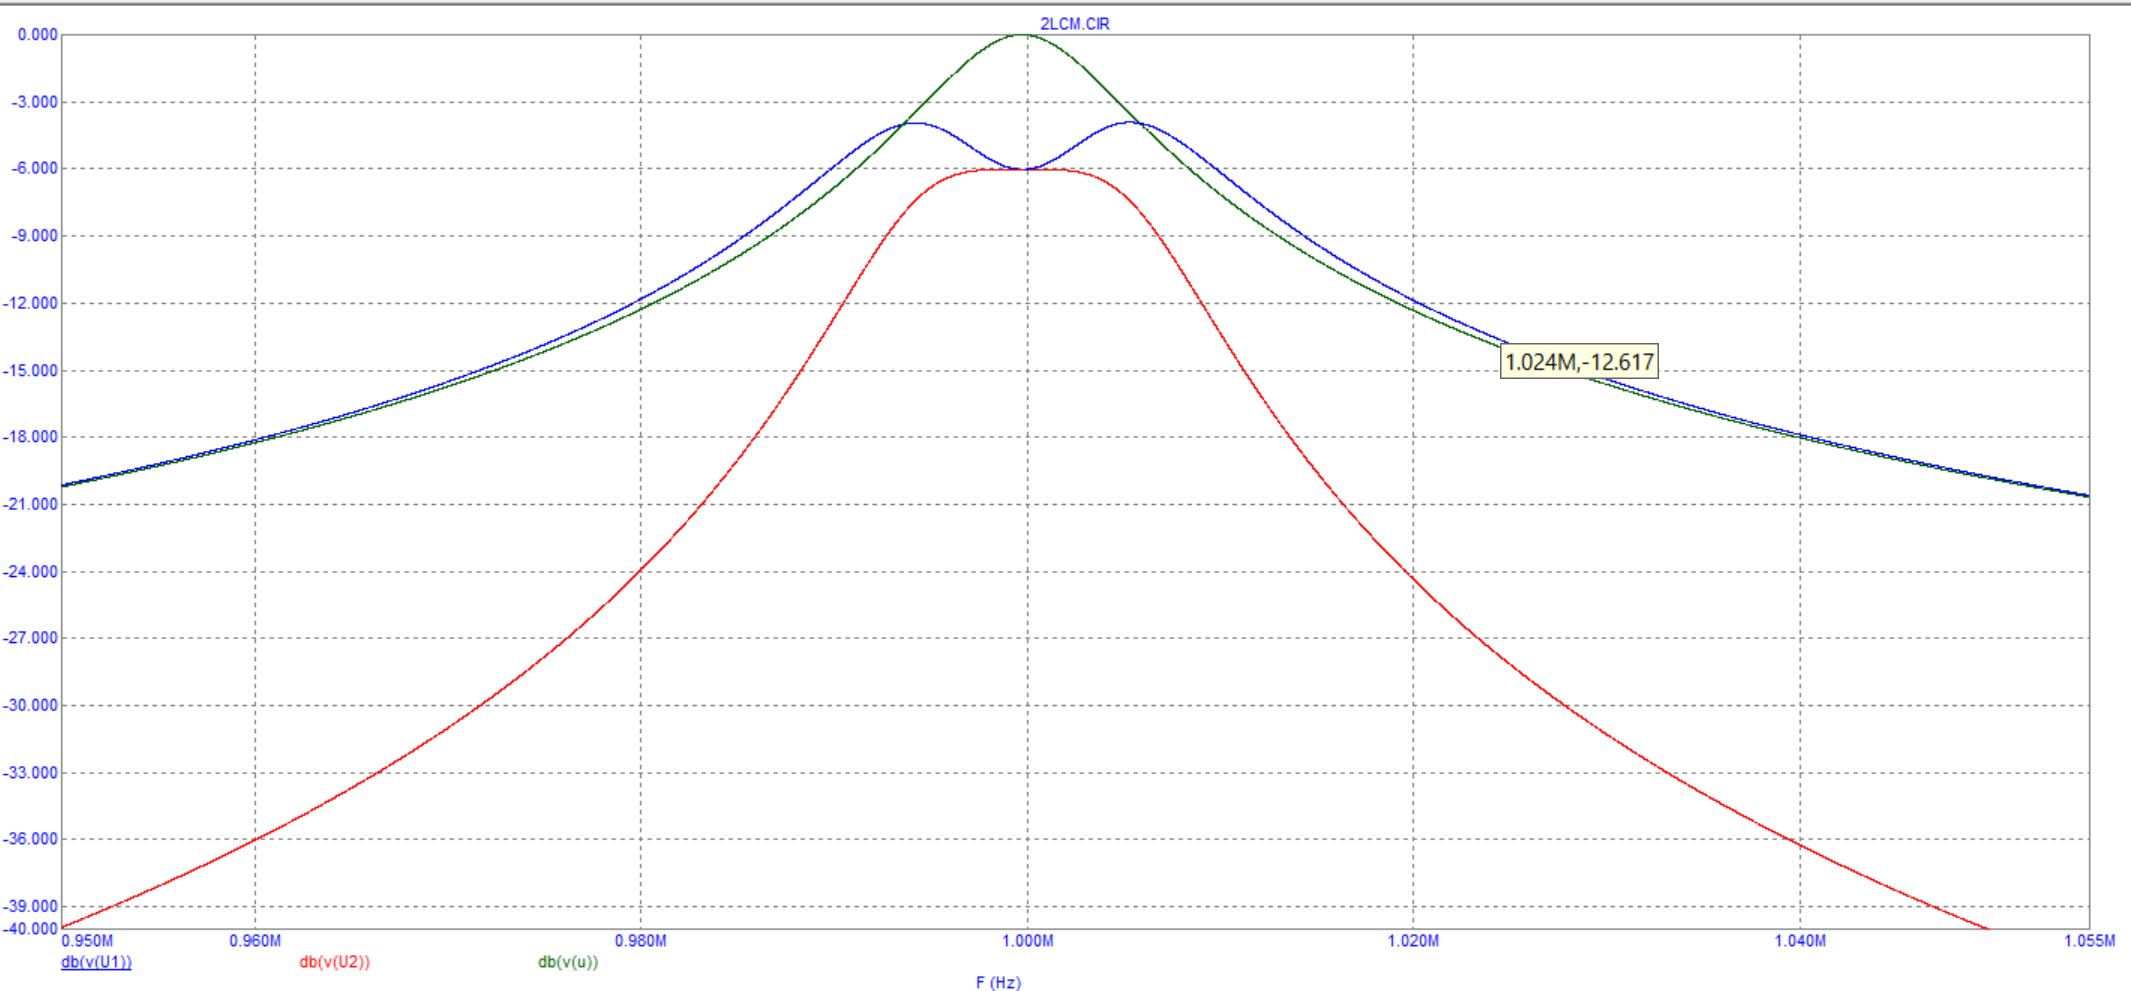
\includegraphics[scale = 0.4]{images/plot5_1.png}
\caption{Схема с начальными характеристиками}
\label{fig:Image1}
\end{figure}

Измерим уровни затухания критической кривой при сдвигах по частоте на декаду $F_0$, то есть на $\pm 10 F_0 = \pm 50k$ (затухание - $-34 \frac{dB}{\text{дек}_{F_0}}$). Варьируя сопротивление потерь эталонного контура $R = [60k, 80k | 5k]$, выясним, что при добротности $Q = 68.6$ ($R = 70k, \bigtriangleup f = 14.557k$) его полоса сравнивается с полосой двухконтурной системы. Измерим затухание, вносимое эталонным котуром с этой добротостью при расстройках на декаду $F_0$ (затухание - $- 16.7 \frac{dB}{\text{дек}_{F_0}}$). Оценим выигрыш двухконтурной системы по затуха-
нию: выигрыш $\simeq$ 2 раза.

\begin{figure}[h!]
\centering
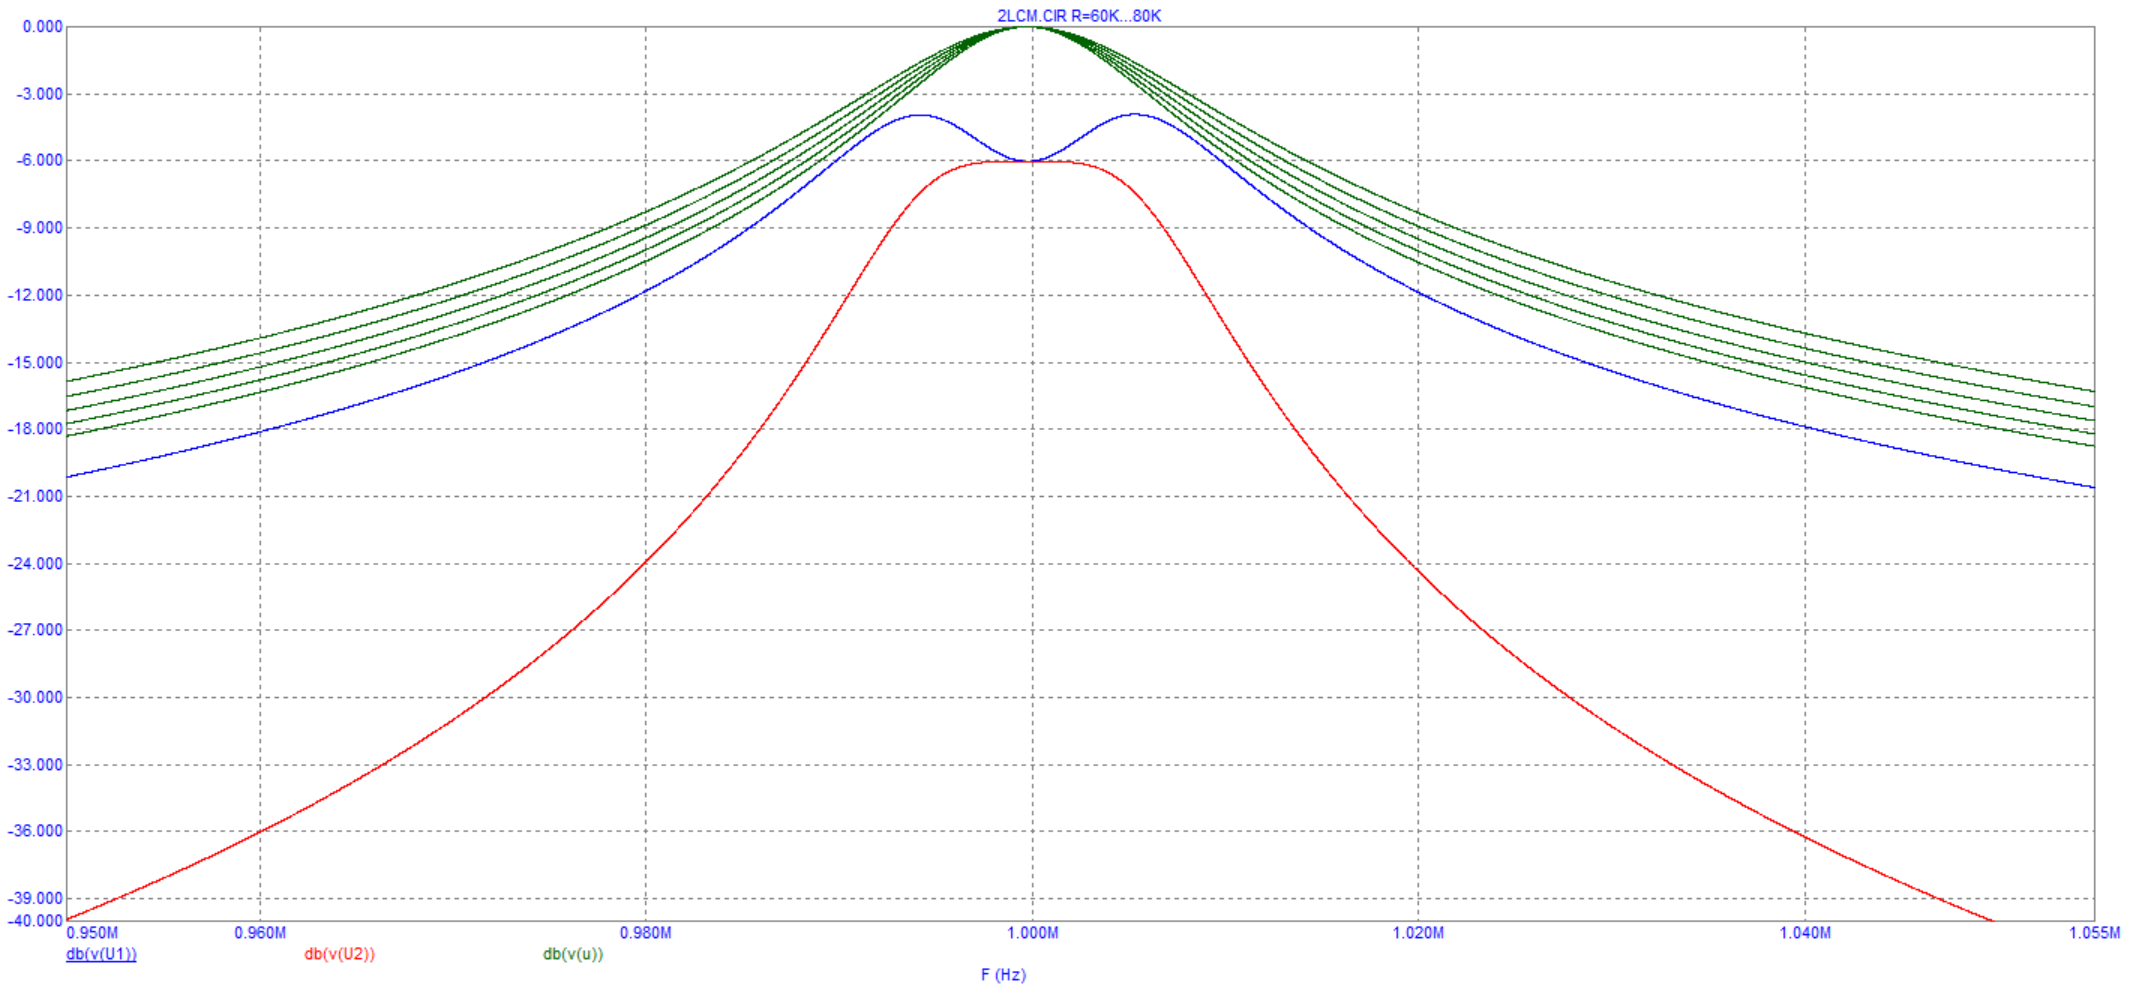
\includegraphics[scale = 0.4]{images/plot5_2.png}
\caption{$К = [60k, 80k | 5k]$}
\label{fig:Image1}
\end{figure}

\newpage

\item Изучим поведение резонансных кривых при $F = [0.5, 1 | 0.1]$. 

\begin{figure}[h!]
\centering
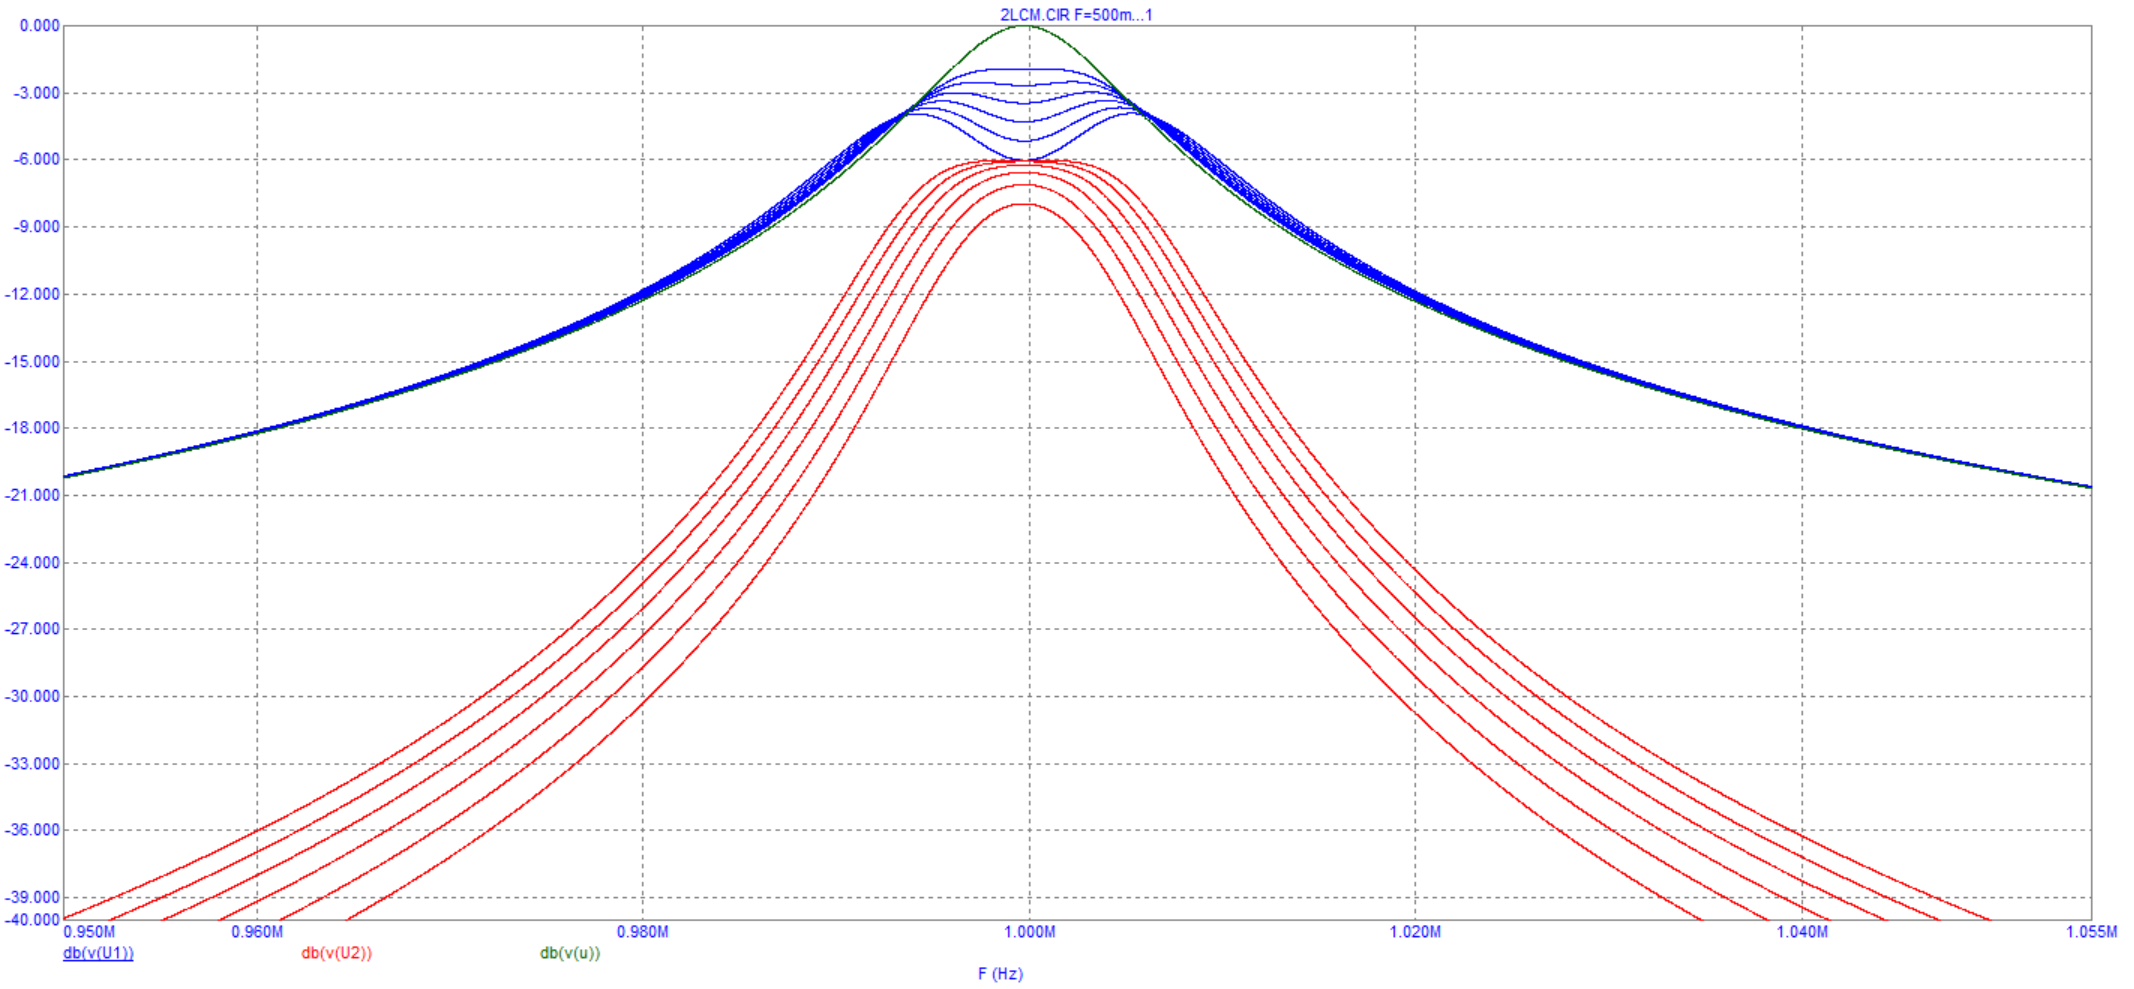
\includegraphics[scale = 0.4]{images/plot6_1.png}
\caption{$F = [0.5, 1 | 0.1]$}
\label{fig:Image1}
\end{figure}

Найдём значение $F = [0.65, 0.75 | 0.05]$, при котором полоса двухконтурной системы по критическому уровню -9dB сравнивается с полосой 10$k$ эталонного контура: $F = 0.75$. При этом значении $F$ оценим выигрыш по затуханию при расстройке на декаду $F_0$ двухконтурной системы по сравнению с эталоном: у эталона - $-19.75 \frac{dB}{\text{дек}_{F_0}}$, у двухконтурной системы – $-36.45 \frac{dB}{\text{дек}_{F_0}}$ $\Longrightarrow$ выигрыш $\approx$ 2 раза.

\begin{figure}[h!]
\centering
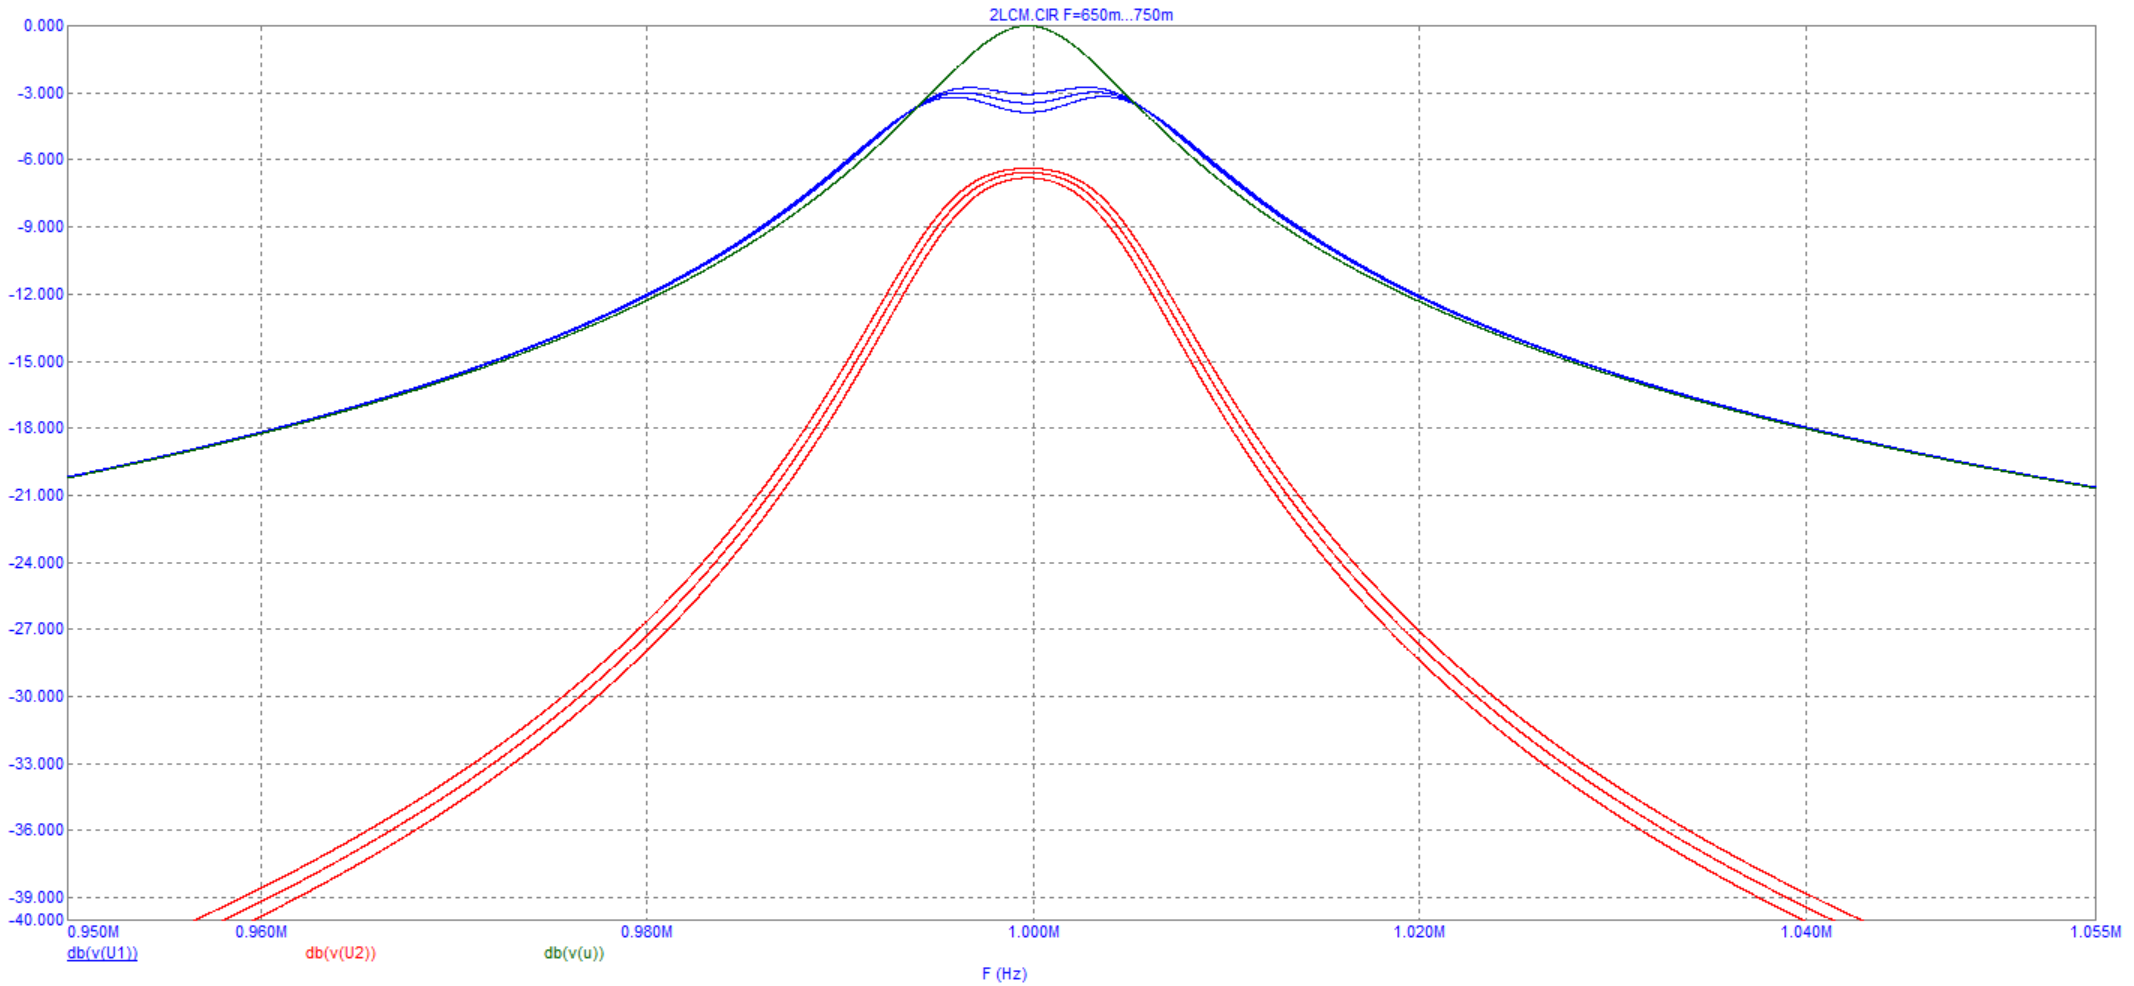
\includegraphics[scale = 0.4]{images/plot6_2.png}
\caption{$F = [0.65, 0.75 | 0.05]$}
\label{fig:Image1}
\end{figure}

\newpage

\item Измерим значение $F$ из диапазона $F = [2.2, 2.6 | 0.1]$, при котором провал во втором контуре касается сверху критического уровня -9dB. 
$F = 2.4$: при этом значении $F$ измерим ширину полосы $\bigtriangleup\omega$ двухконтурной системы по уровню -9dB ($\bigtriangleup \omega$) и уровни затухания при расстройках на декаду $F_0$ (у эталона - $-20 \frac{dB}{\text{дек}}$, у двухконтурной системы - $-23 \frac{dB}{\text{дек}}$). Варьированием сопротив-
ления эталонного контура $R$ добьёмся совпадения его полосы с полосой двухконтурной системы и измерим уровни затухания, вносимого контуром ($-18.322 \frac{dB}{\text{дек}}$). ($R = 140k$).

\begin{figure}[h!]
\centering
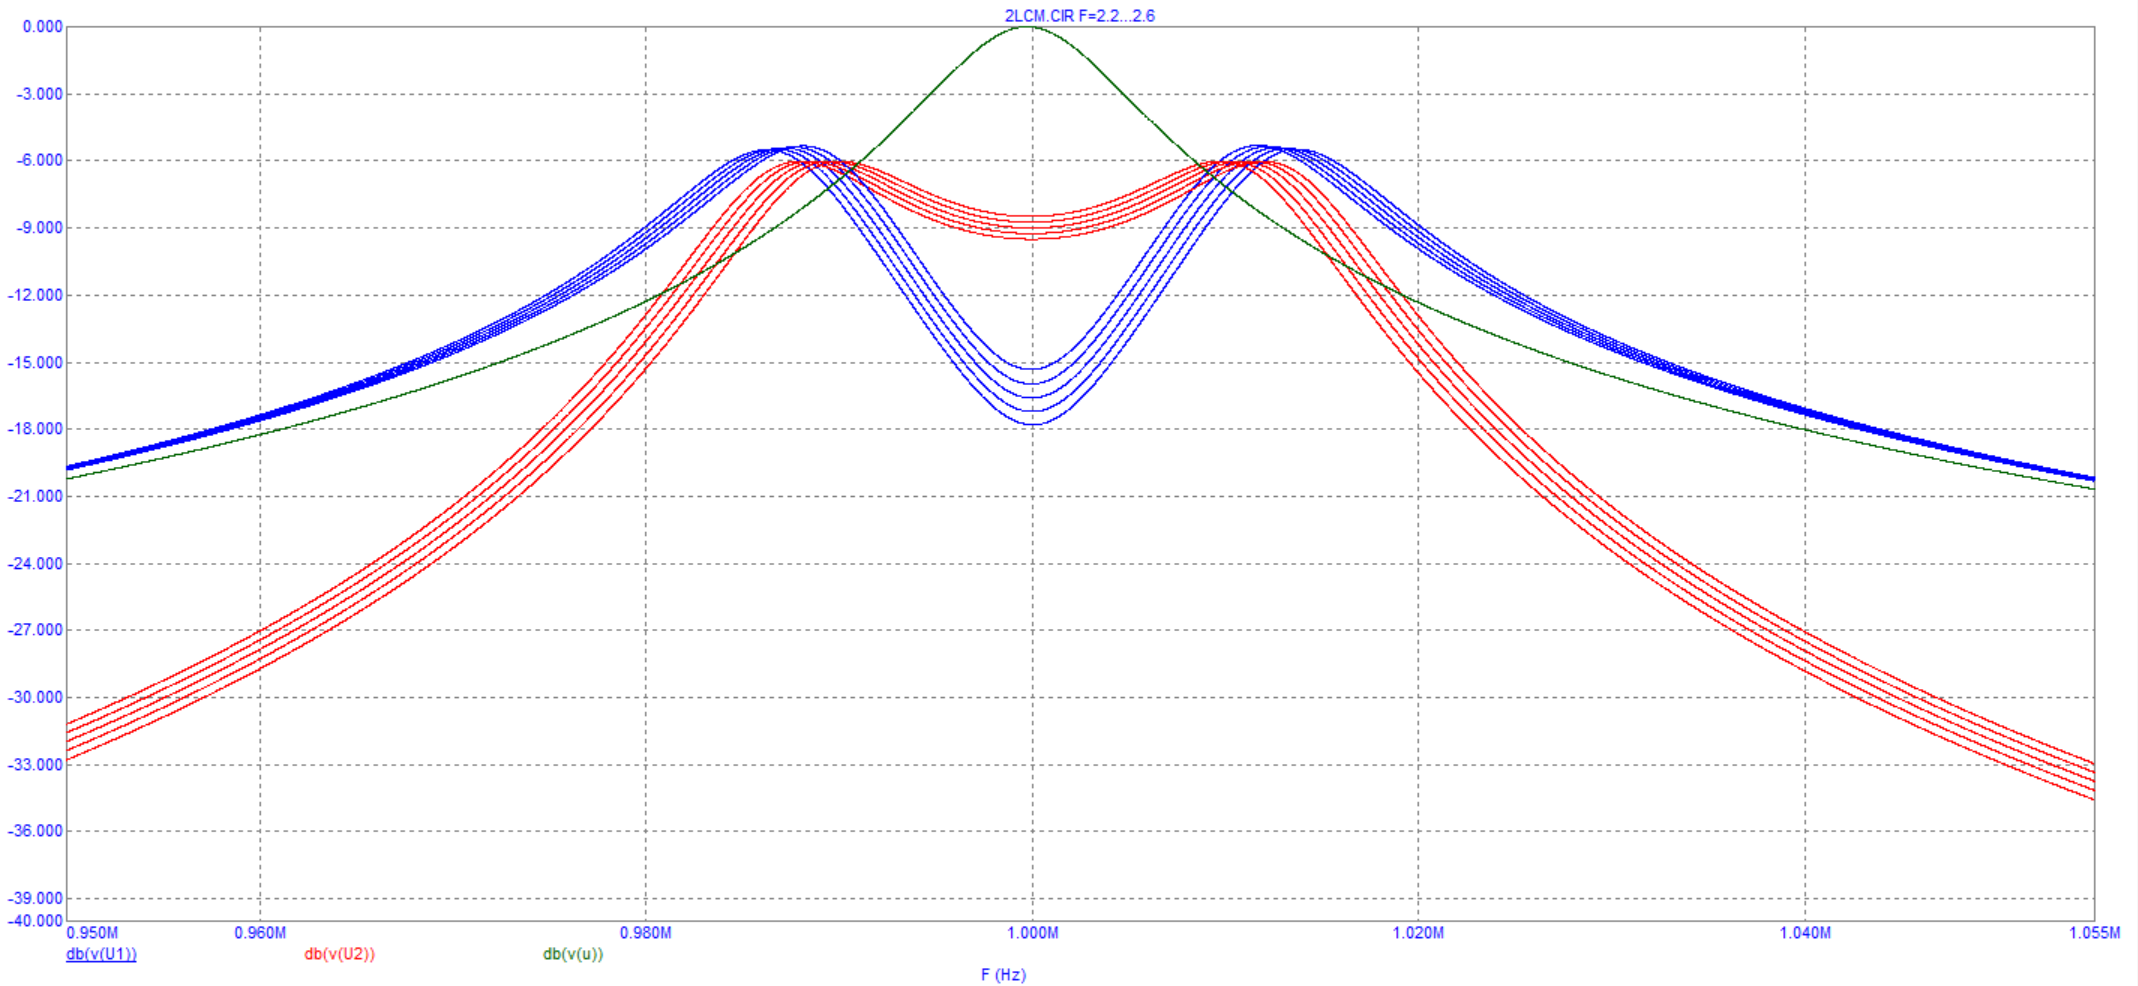
\includegraphics[scale = 0.4]{images/plot7_1.png}
\caption{$F = [2.2, 2.6 | 0.1]$}
\label{fig:Image1}
\end{figure}

\newpage

\item Изучим зависимость уровней затухания от $F = [1,5.5|1.5]$. Занесём
результаты в таблицу 2.

\begin{figure}[h!]
\centering
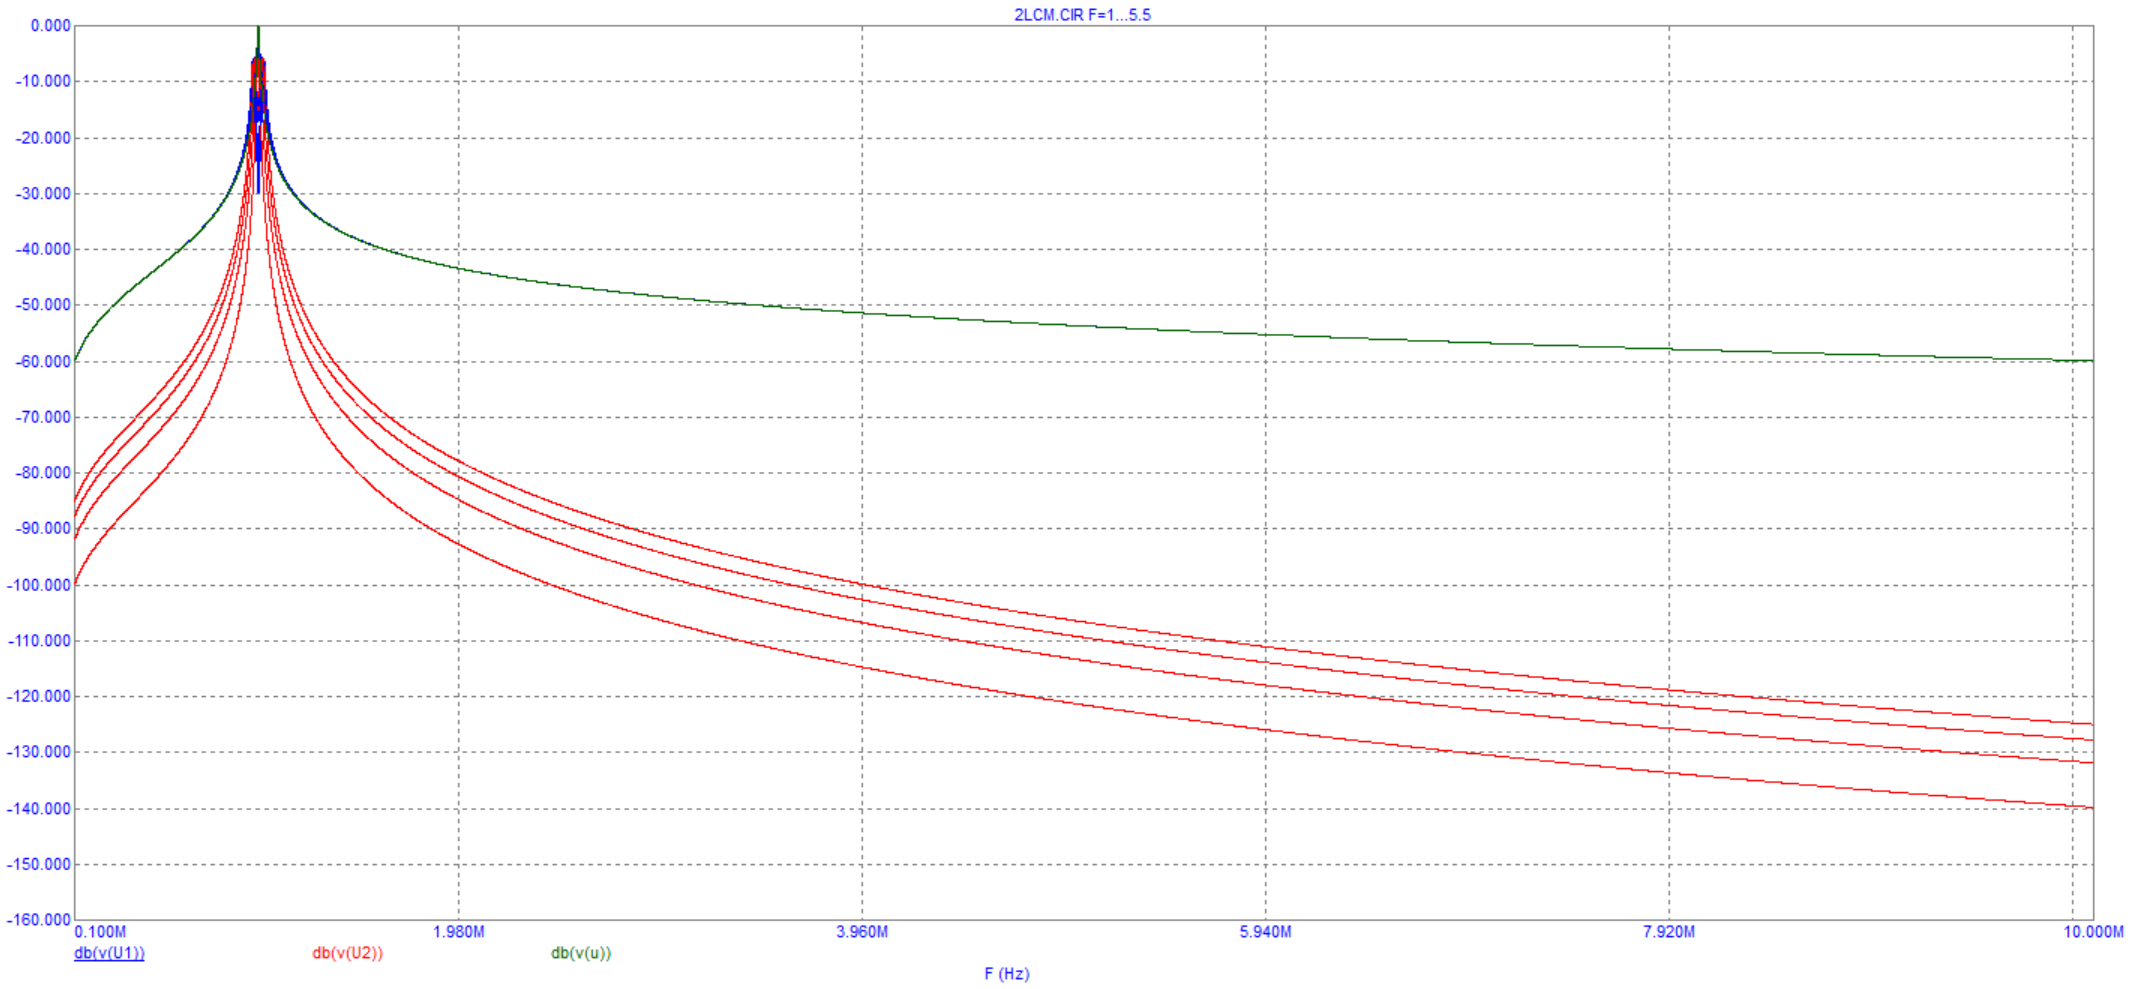
\includegraphics[scale = 0.4]{images/plot8_1.png}
\caption{$F = [1,5.5|1.5]$}
\label{fig:Image1}
\end{figure}

\begin{tabular}{|c|c|c|}
\hline 
F & f = 100k & f = 10Meg \\ 
\hline 
1 & -94 & -133 \\ 
\hline 
2.5 & -85 & -126 \\ 
\hline 
4 & -82 & -122 \\ 
\hline 
5.5 & -79 & -119 \\ 
\hline 
\end{tabular} 

Установим добротность эталонного контура равной $\frac{Q}{\sqrt{2}}$ (сопротивление потерь $R = [70k,70k|1k])$, оценим выигрыш в затухании двухконтурной системы с $F = 1$ по сравнению с эталонным контуром с той же шириной полосы. Он равен $f = 100k \Rightarrow 40\frac{dB}{\text{дек}}$, $f = 10Meg \Rightarrow 80\frac{dB}{\text{дек}}$.

\begin{figure}[h!]
\centering
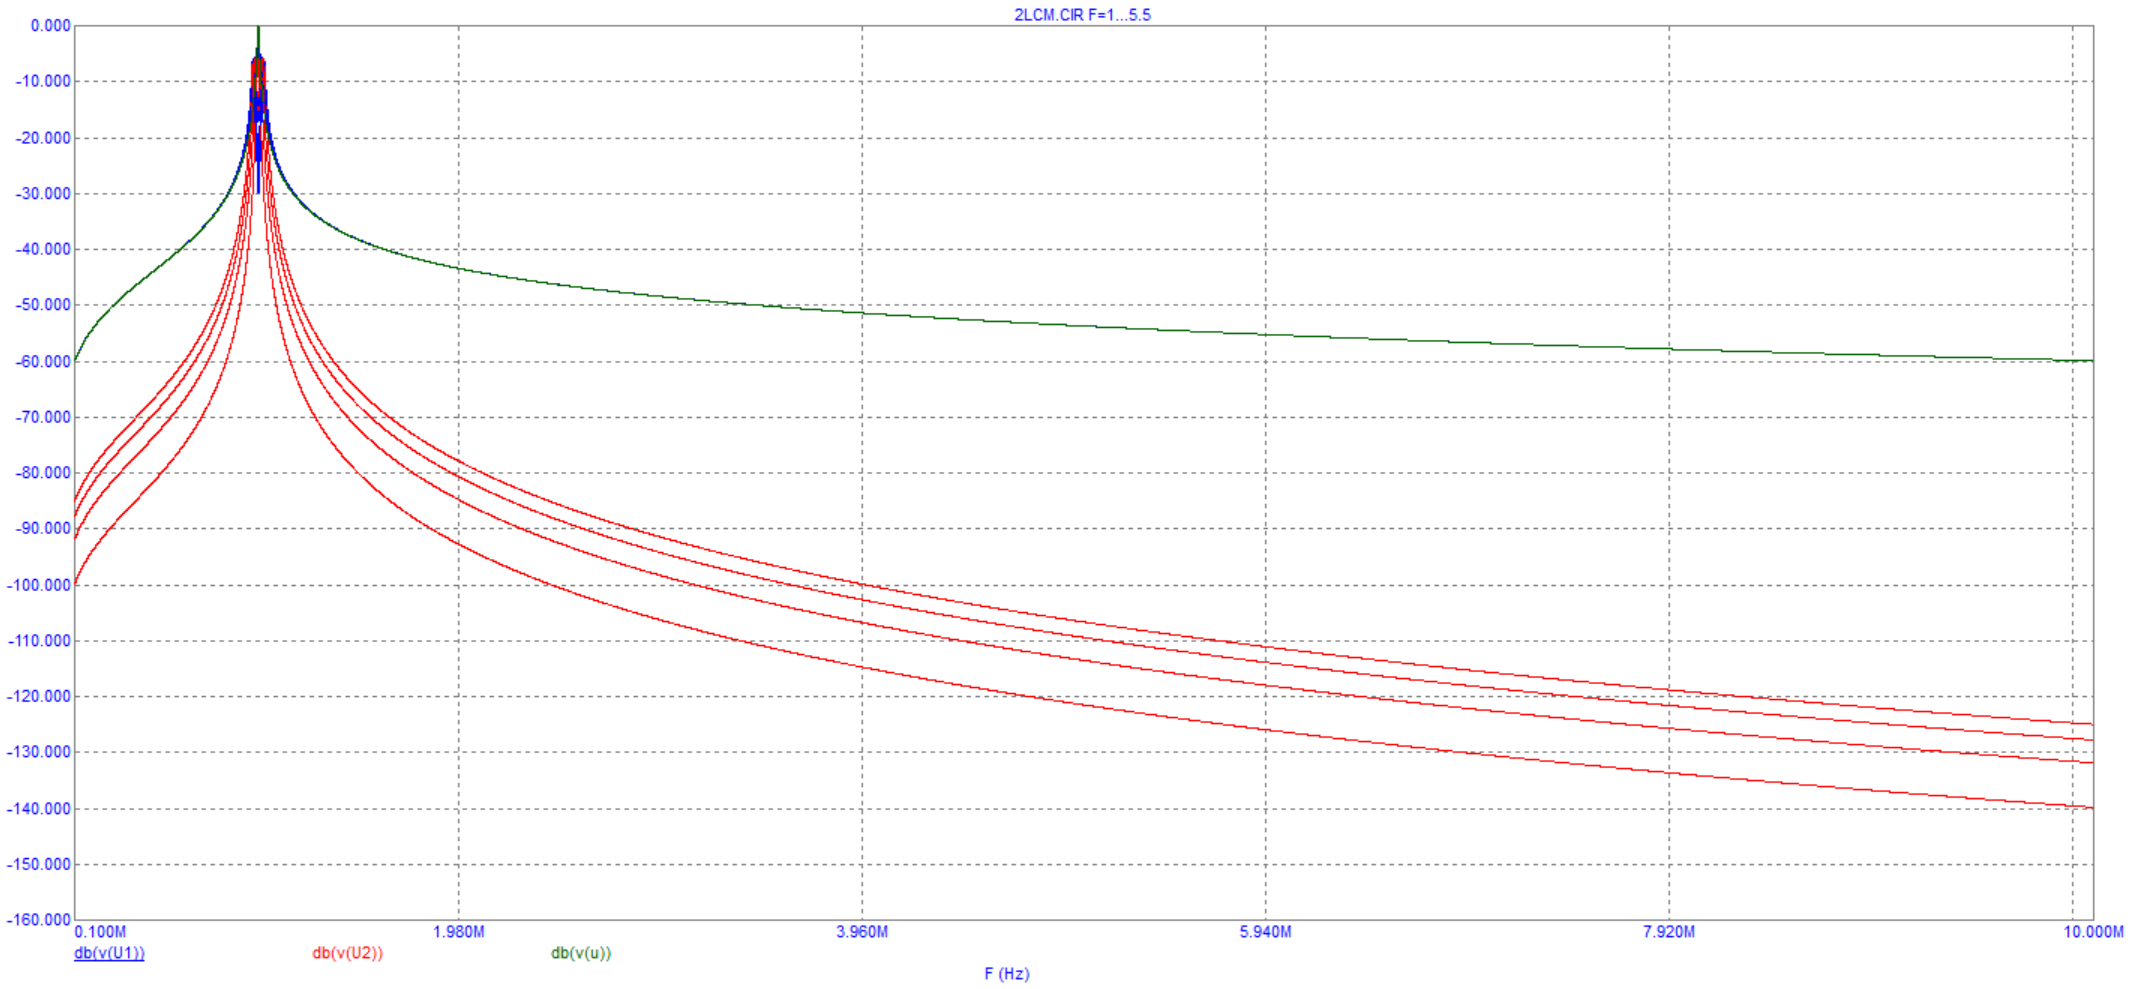
\includegraphics[scale = 0.4]{images/plot8_1.png}
\caption{$R = [70k,70k|1k], Q = 70, F = 1$}
\label{fig:Image1}
\end{figure}

\newpage

\item Включим плоты 2 и 4 - частотные характеристики и графики вносимых проводимостей. Снимем зависимость пиковых значений вещественной и мнимой частей вносимой проводимости от $F = [0.5, 1 | 0.5]$ и $F = [1,2|1]$. Проверим формулу $Re(Y) = \frac{F^2}{Q_{\rho}}$. 

\begin{figure}[h!]
\centering
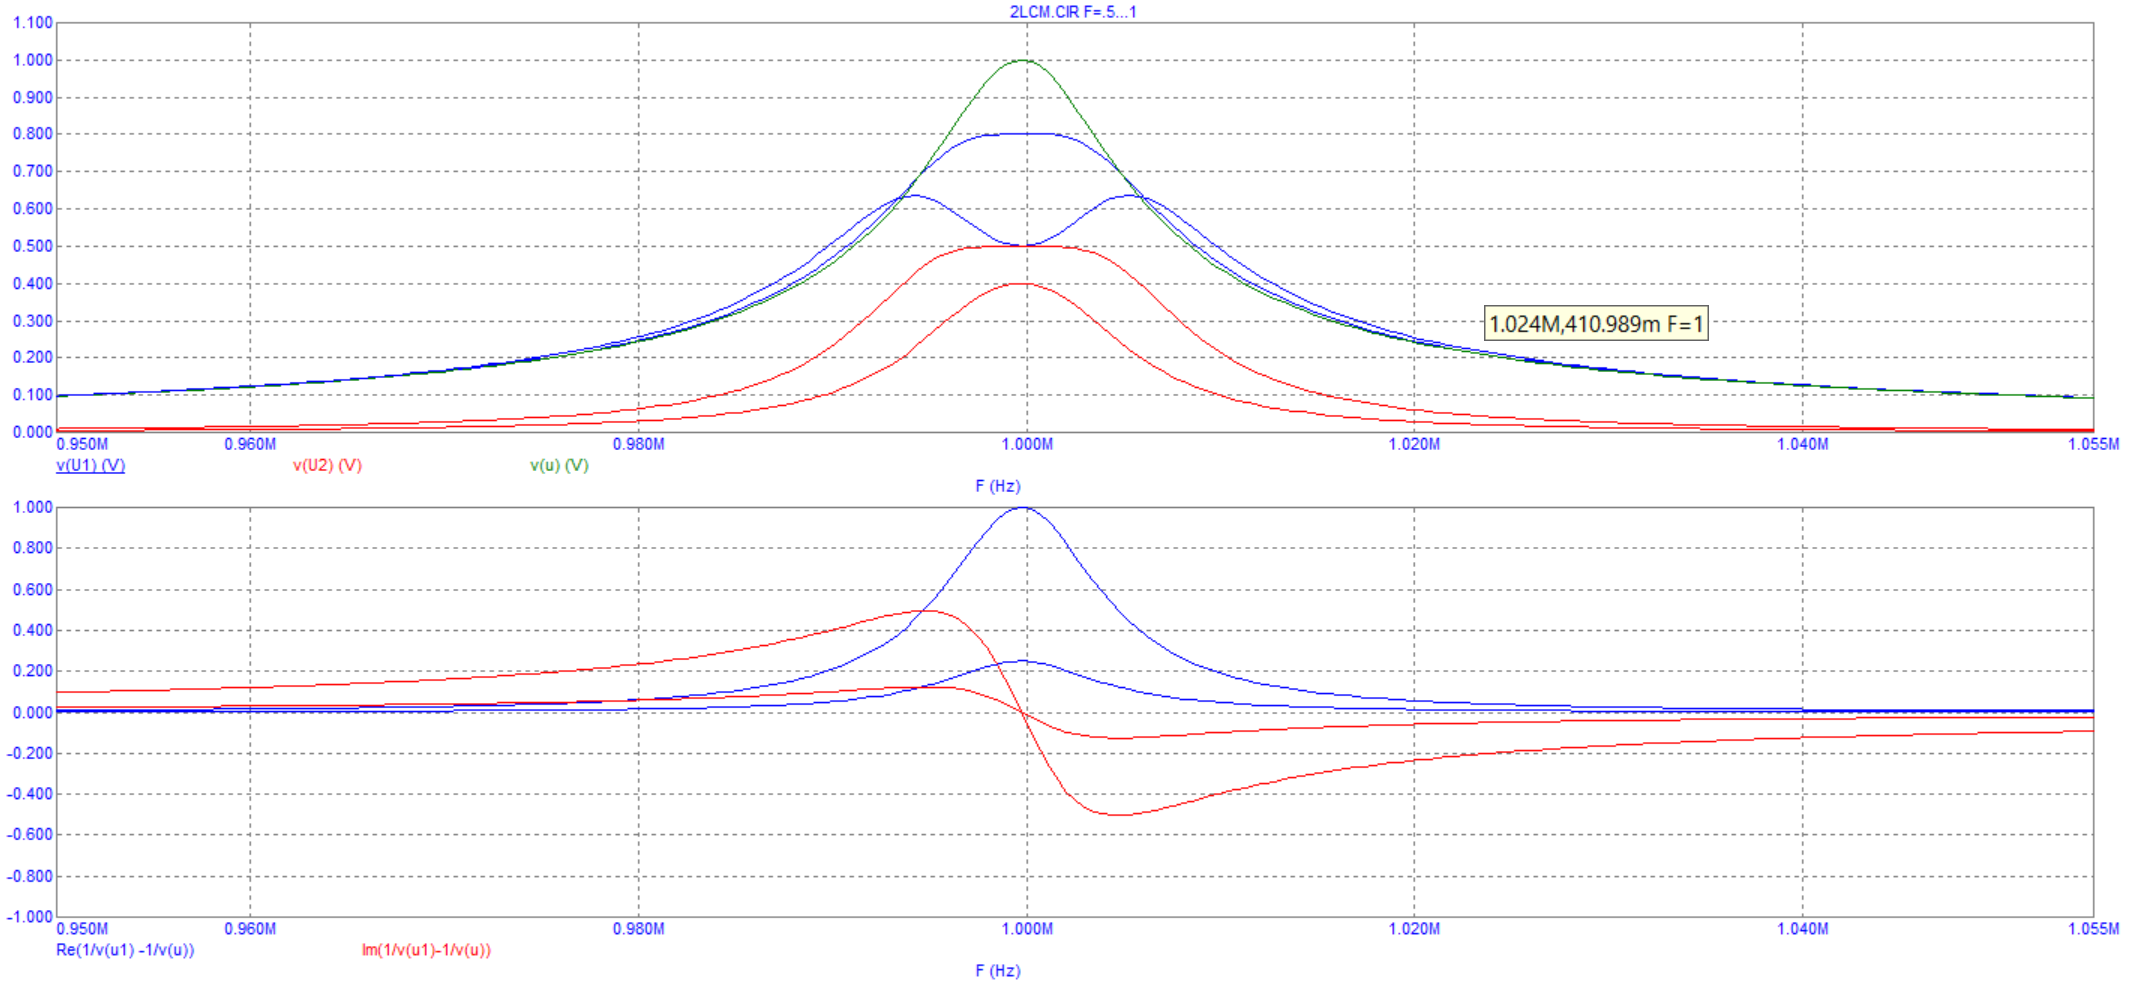
\includegraphics[scale = 0.4]{images/plot9_1.png}
\caption{$F = [0.5, 1 | 0.5]$}
\label{fig:Image1}
\end{figure}

\begin{figure}[h!]
\centering
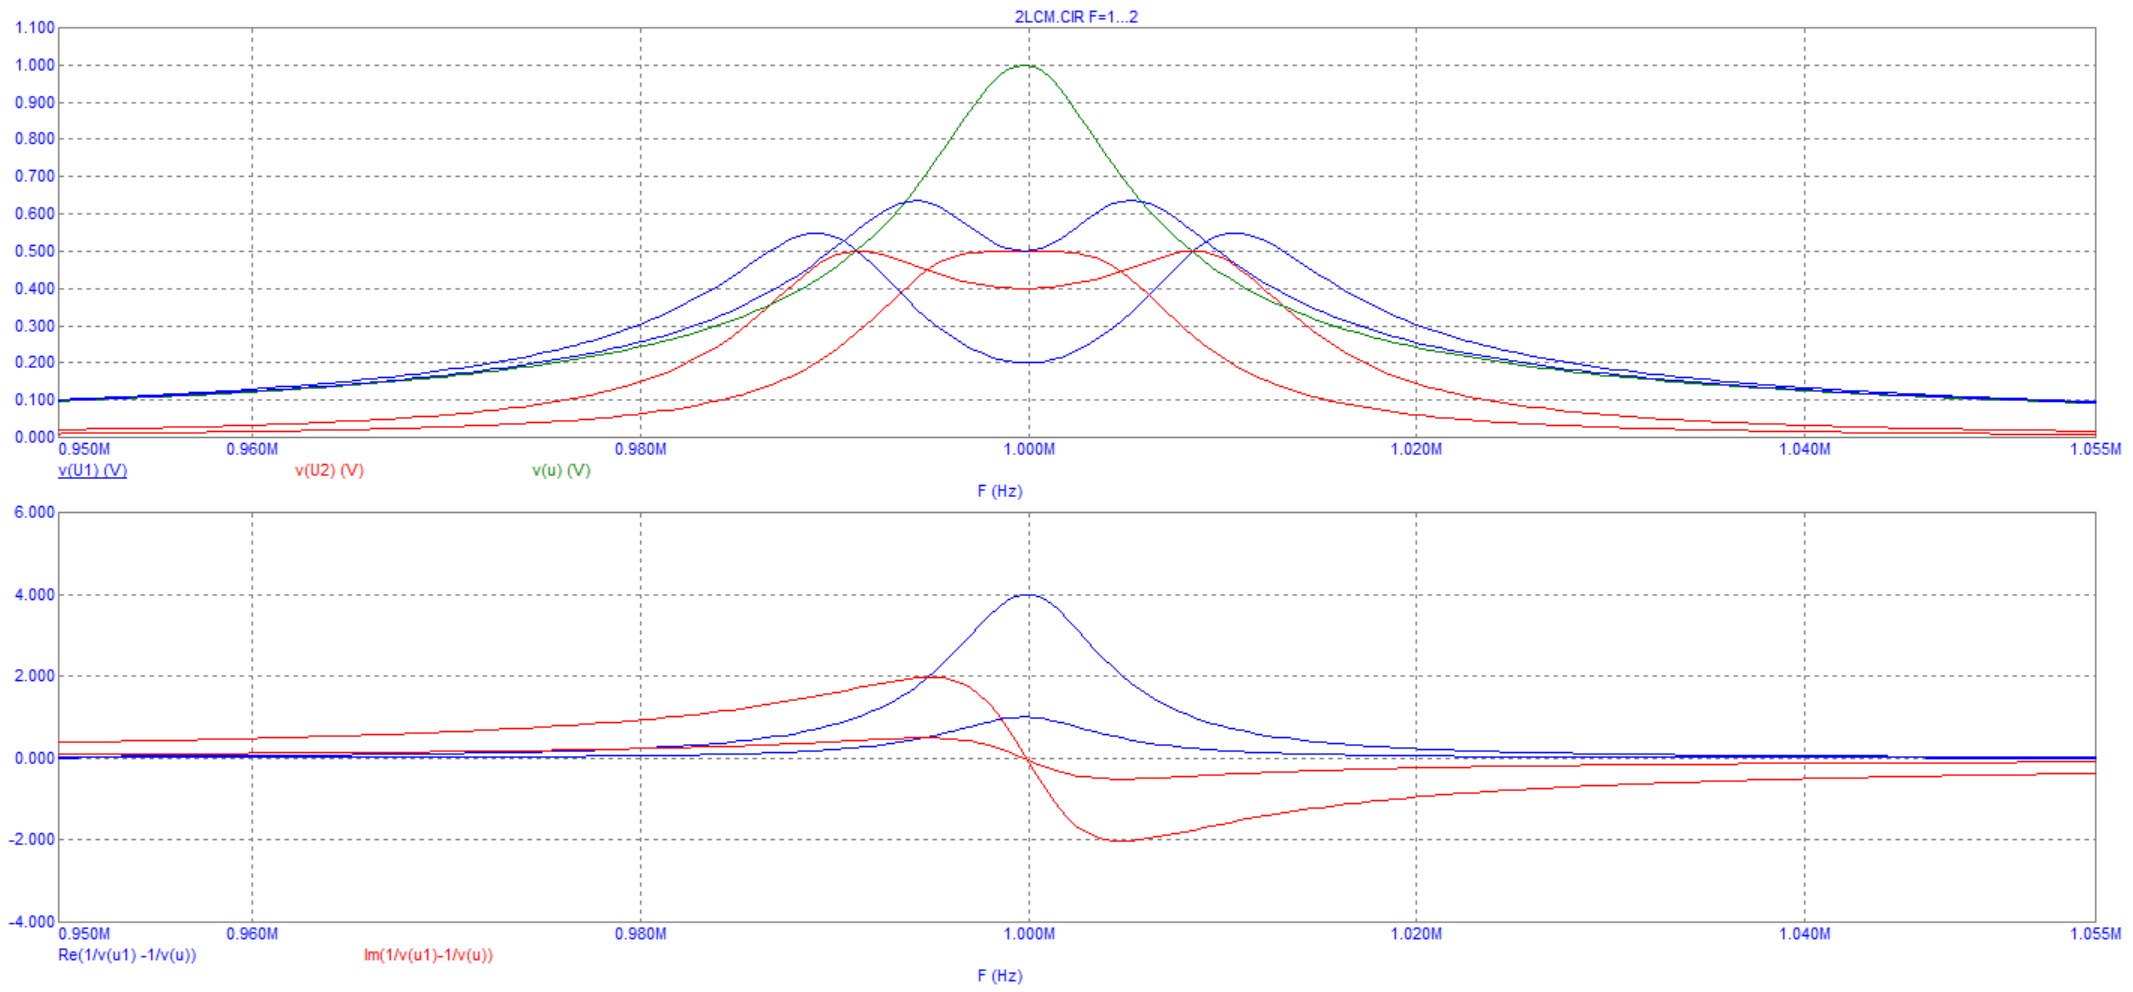
\includegraphics[scale = 0.4]{images/plot9_2.png}
\caption{$F = [1,2|1]$}
\label{fig:Image1}
\end{figure}

\begin{center}
\begin{tabular}{|c|c|c|}
\hline 
F & Im & Re \\ 
\hline 
2 & 200k & 400k \\ 
\hline 
1 & 50k & 100k \\ 
\hline 
0.5 & 12,5k & 25k \\ 
\hline 
\end{tabular} 
\end{center}

Оценим значения вносимых емкостей $\varepsilon C$ при $F = 0.5,1,2$, зная, что:

\[\omega \varepsilon C \simeq \frac{\varepsilon}{\rho} = \frac{\varepsilon}{1k},\]

а уровень на графике дает значение в $100 \varepsilon$.

\begin{center}
\begin{tabular}{|c|c|}
\hline 
F & $\varepsilon C$ \\ 
\hline 
0.5 & 12.5 $\varepsilon$ \\ 
\hline 
1 & 50 $\varepsilon$\\ 
\hline 
2 & 200 $\varepsilon$\\ 
\hline 
\end{tabular} 
\end{center}

\newpage

\item В режиме \textit{Transient} проанализируем переходные характеристики до напряжений на первом и втором контурах при $F = 1$.

\begin{figure}[h!]
\centering
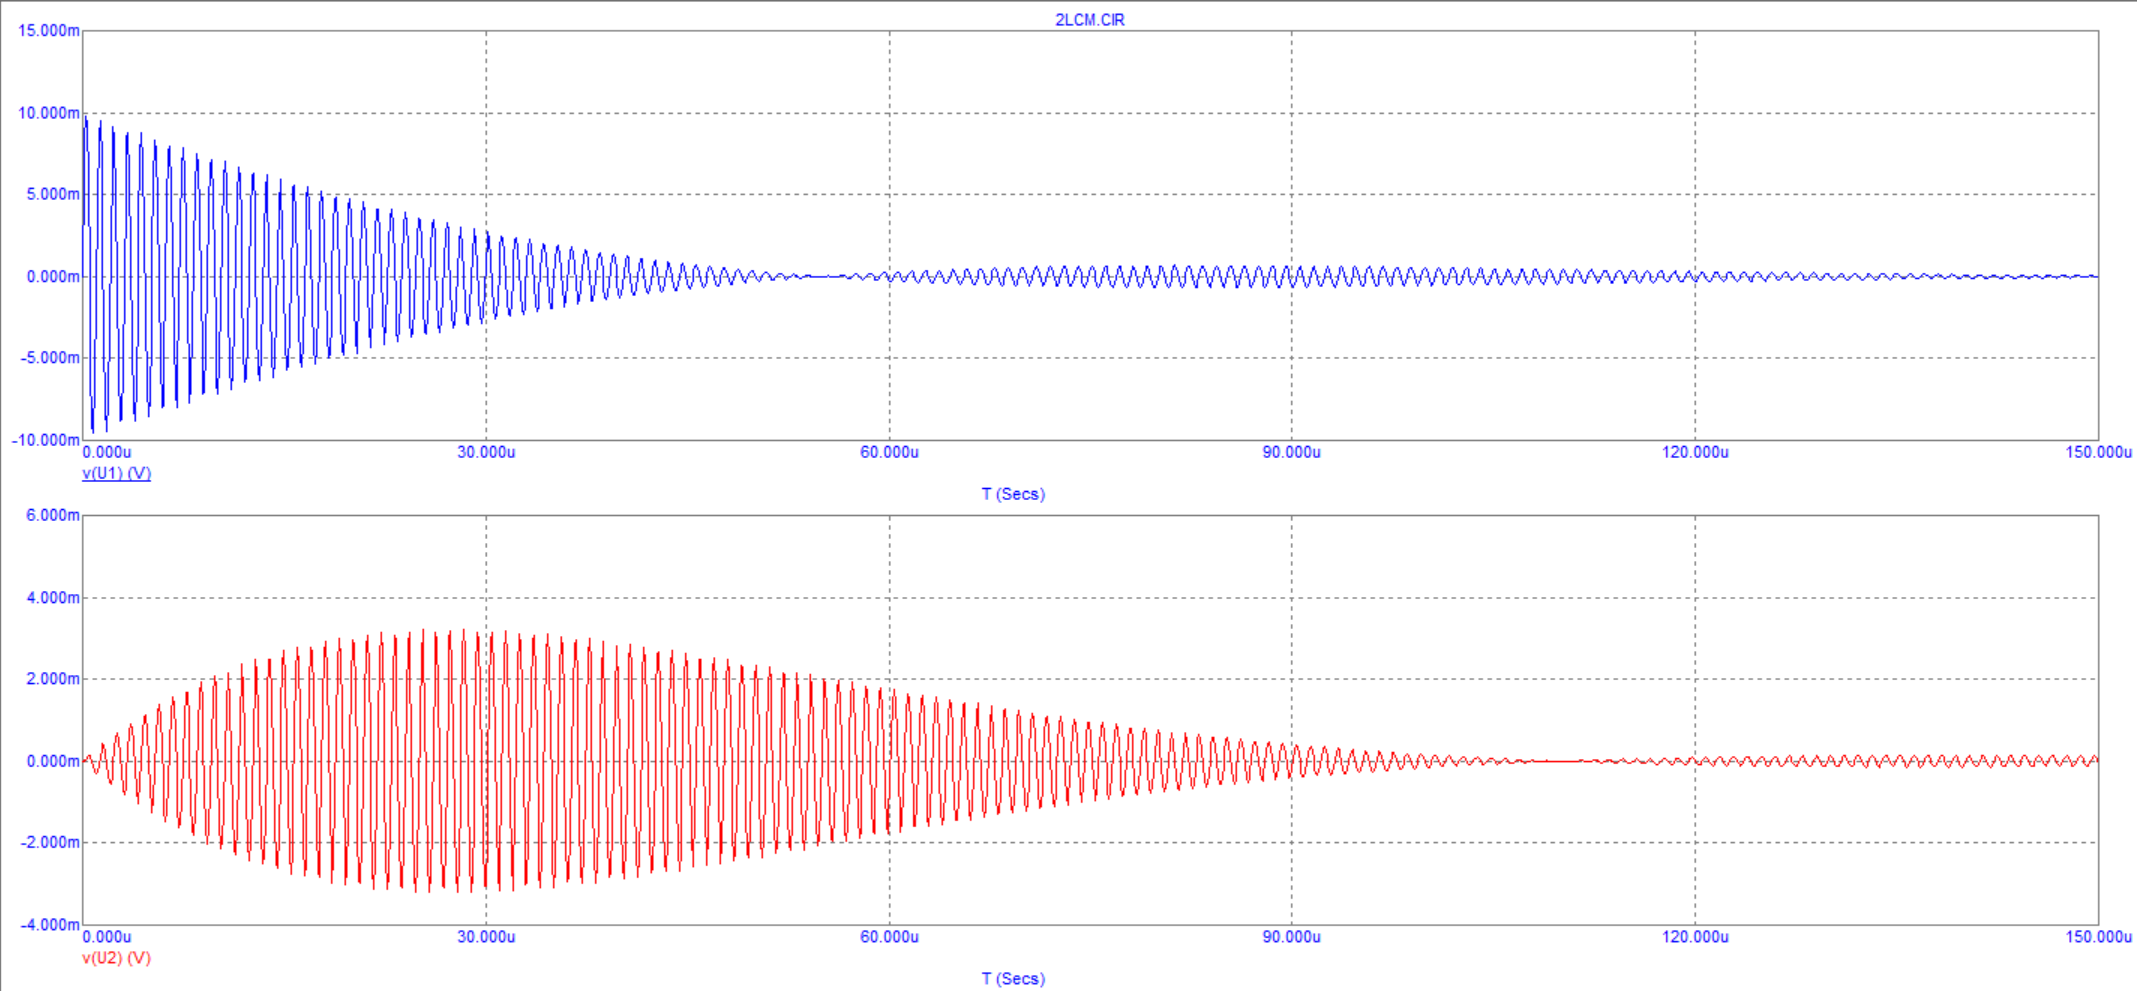
\includegraphics[scale = 0.4]{images/plot10_1.png}
\caption{$F = 1$}
\label{fig:Image1}
\end{figure}

Установим $F = 0.1$. Измерим постоянную времени $\tau$ экспоненциального спада огибающий напряжения $u_1 \sim e^{-t/\tau}$ до уровня $\frac{1}{e} = 0.37$. $\tau \simeq = 32$ мкс. Следовательно выполняется соотношение:

\[\tau \frac{\pi}{2\pi F_0} \simeq 32 \mu\]

\begin{figure}[h!]
\centering
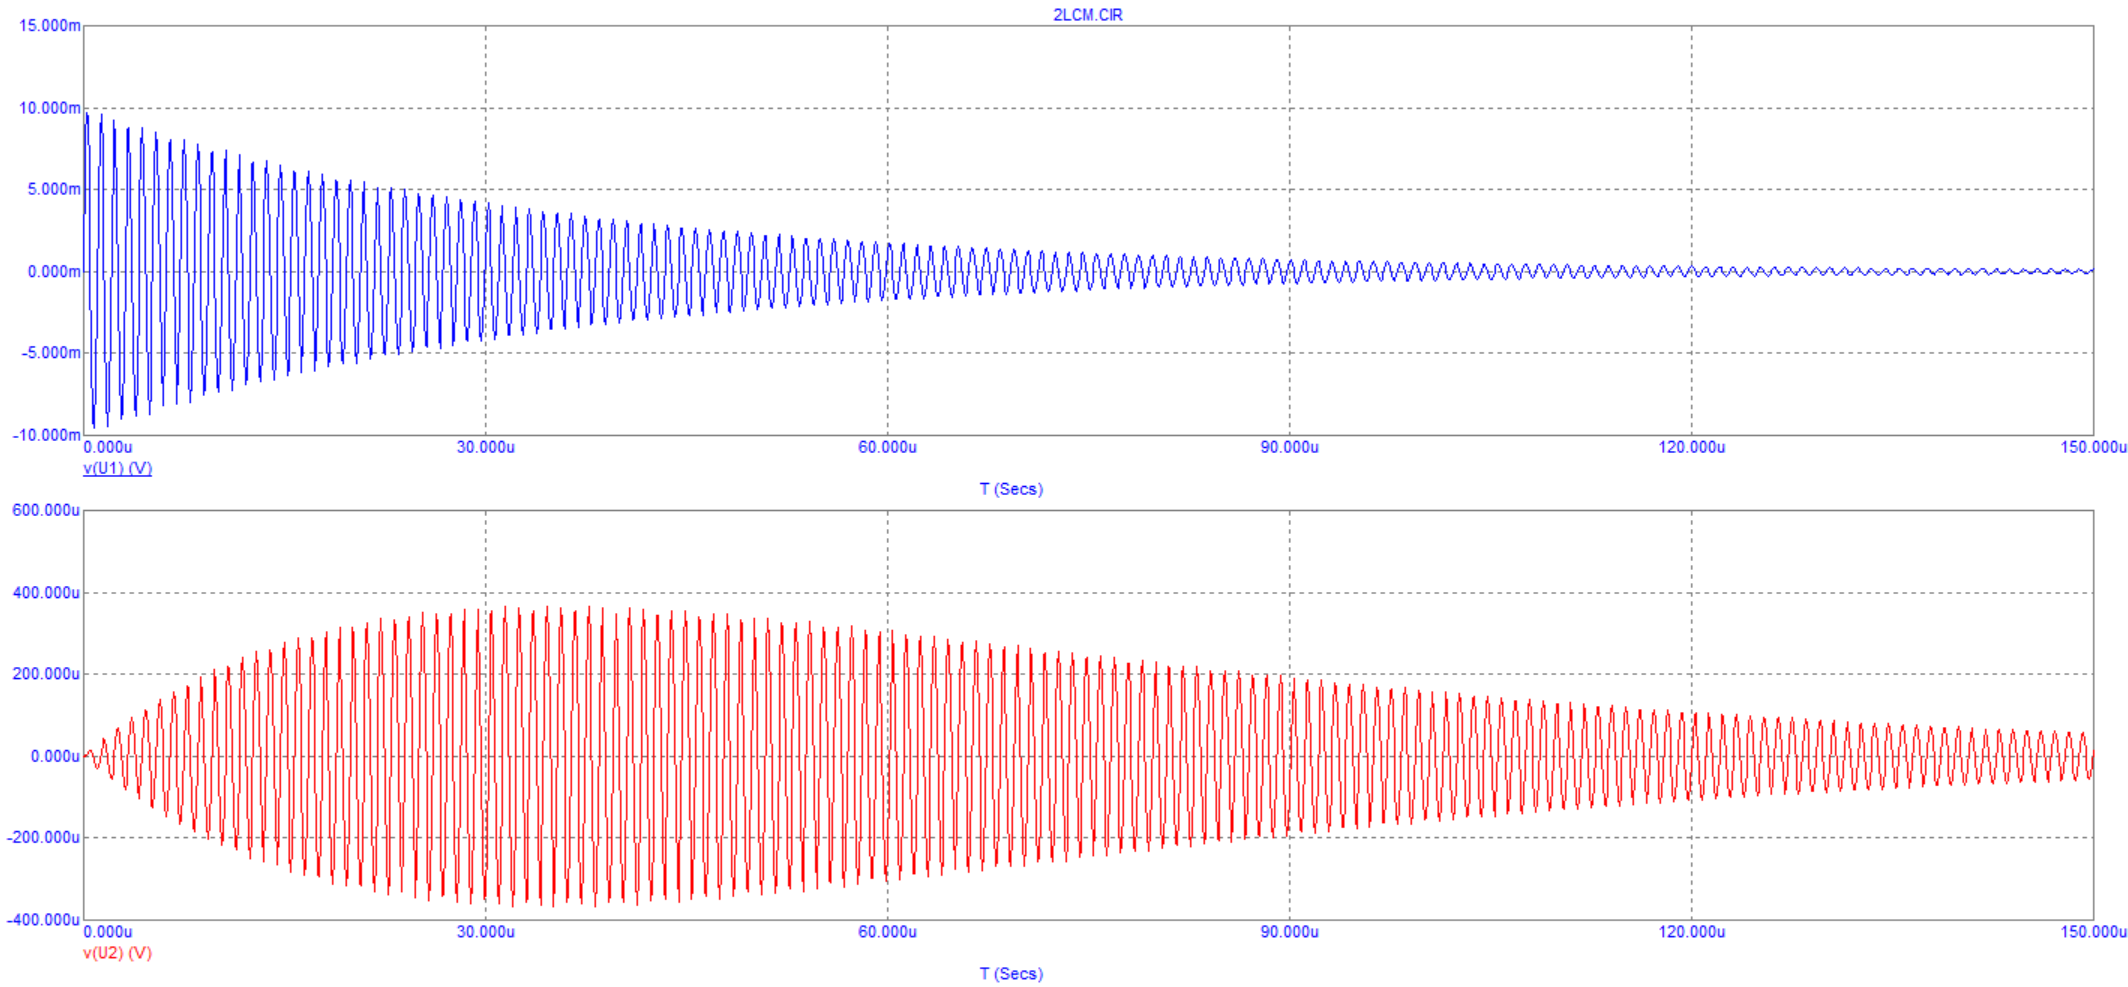
\includegraphics[scale = 0.4]{images/plot10_2.png}
\caption{$F = 0.1$}
\label{fig:Image1}
\end{figure}

Задавая поочередно значения $F = 1;2;4;8$, снимем зависимость от $F$ частоты биений.

\begin{center}
\begin{tabular}{|c|c|c|c|c|}
\hline 
F & 1 & 2 & 4 & 8 \\ 
\hline 
$\tau /2$, мкс & 107 & 54 & 27.6 & 13.1 \\ 
\hline 
$\nu$, кГц & 4.8 & 9.0 & 18.4 & 36 \\ 
\hline 
$FF_0$, кГц & 5 & 10 & 20 & 40 \\
\hline
\end{tabular} 
\end{center}

\newpage

\item Установив диапазон моделирования $[2Meg, 600k]$, исследуем частотные и фазовые характеристики при сильной связи, варьируя $F = [10,70|10]$. 

\begin{figure}[h!]
\centering
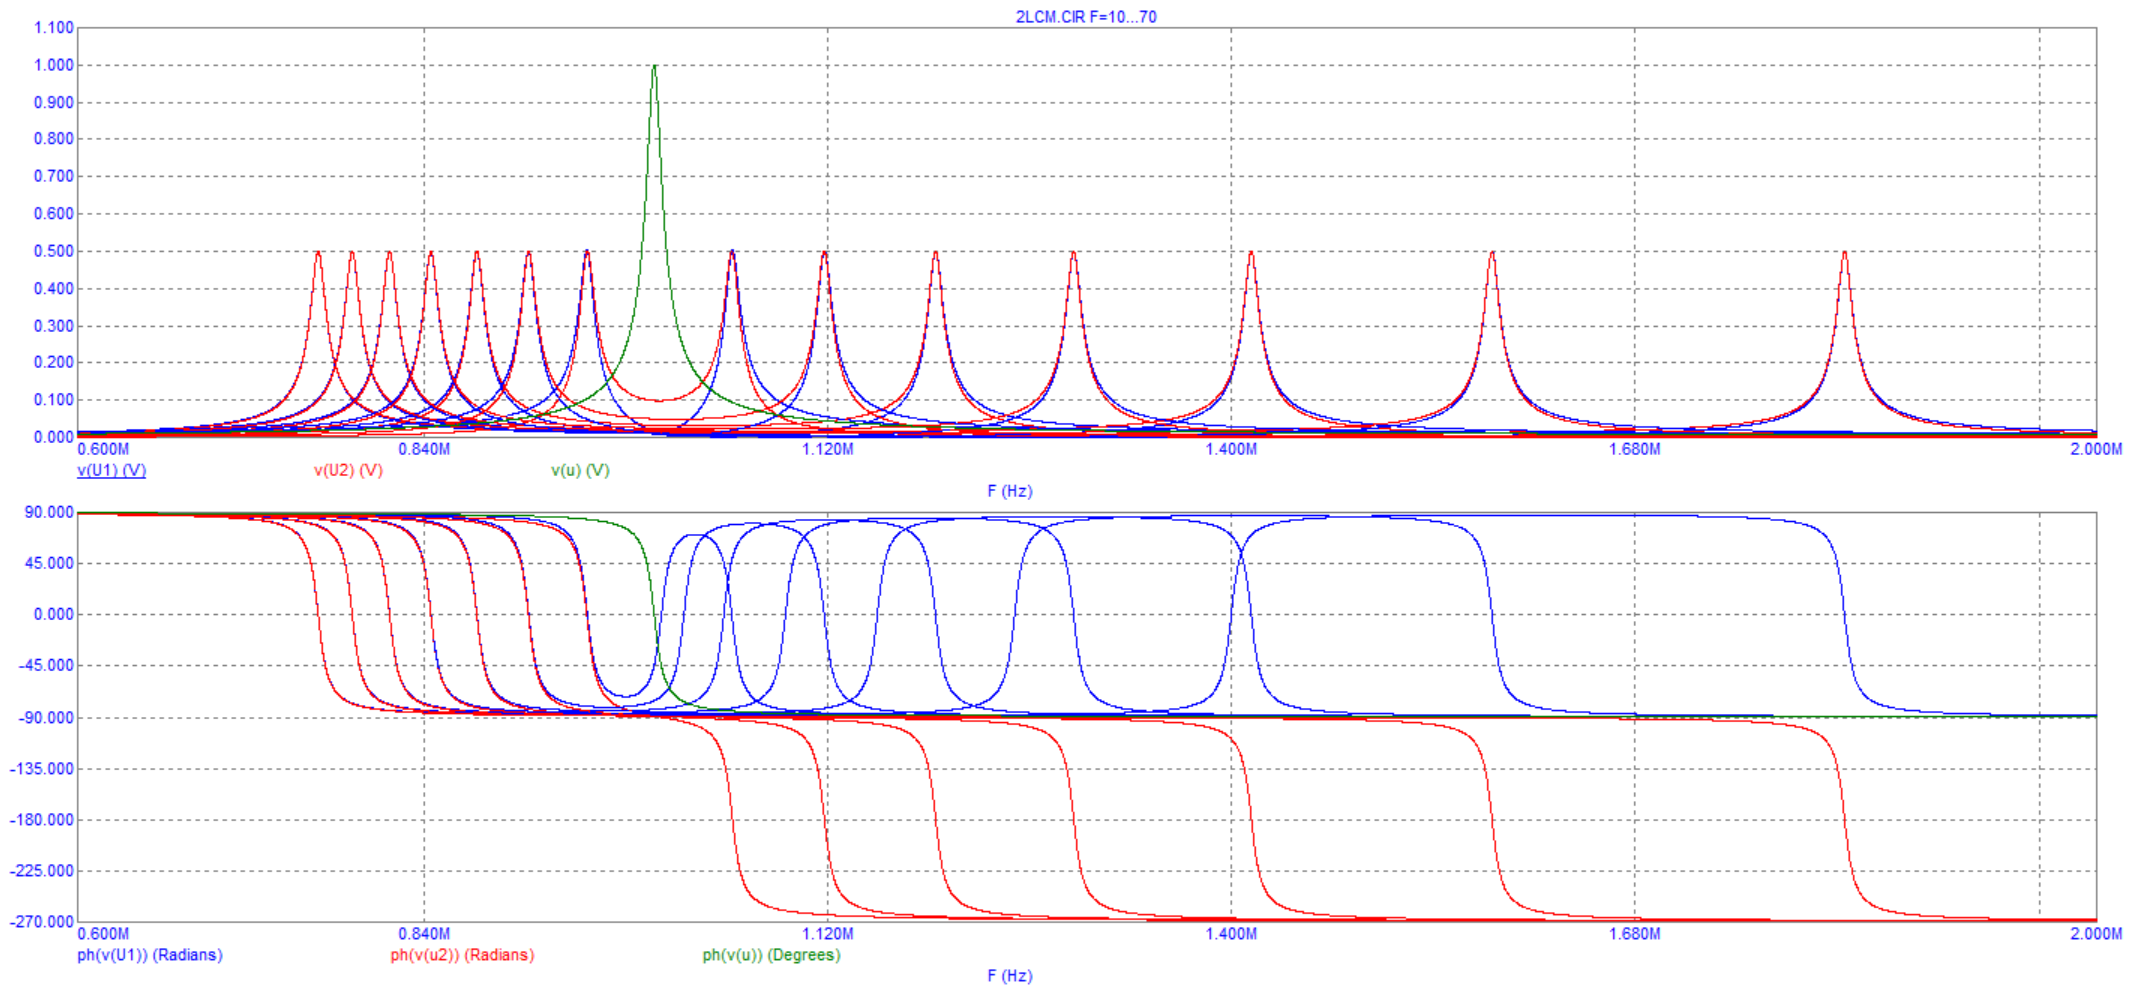
\includegraphics[scale = 0.4]{images/plot11_1.png}
\caption{$F = [10,70|10]$}
\label{fig:Image1}
\end{figure}

Измерим частоты $f_{\pm}$ пиков при $F = 50$. $f_+ = 1,46M$, $F_- = 816,35k$. Убедимся в правильности формулы:

\[f_{\pm} = \frac{f_0}{\sqrt{1\pm k}}\]

Убедимся в том, что при $F \longrightarrow 100$ частота одного пика стремится к $\frac{f_0}{\sqrt{2}}$, а второго уходит в бесконечность.

\begin{figure}[h!]
\centering
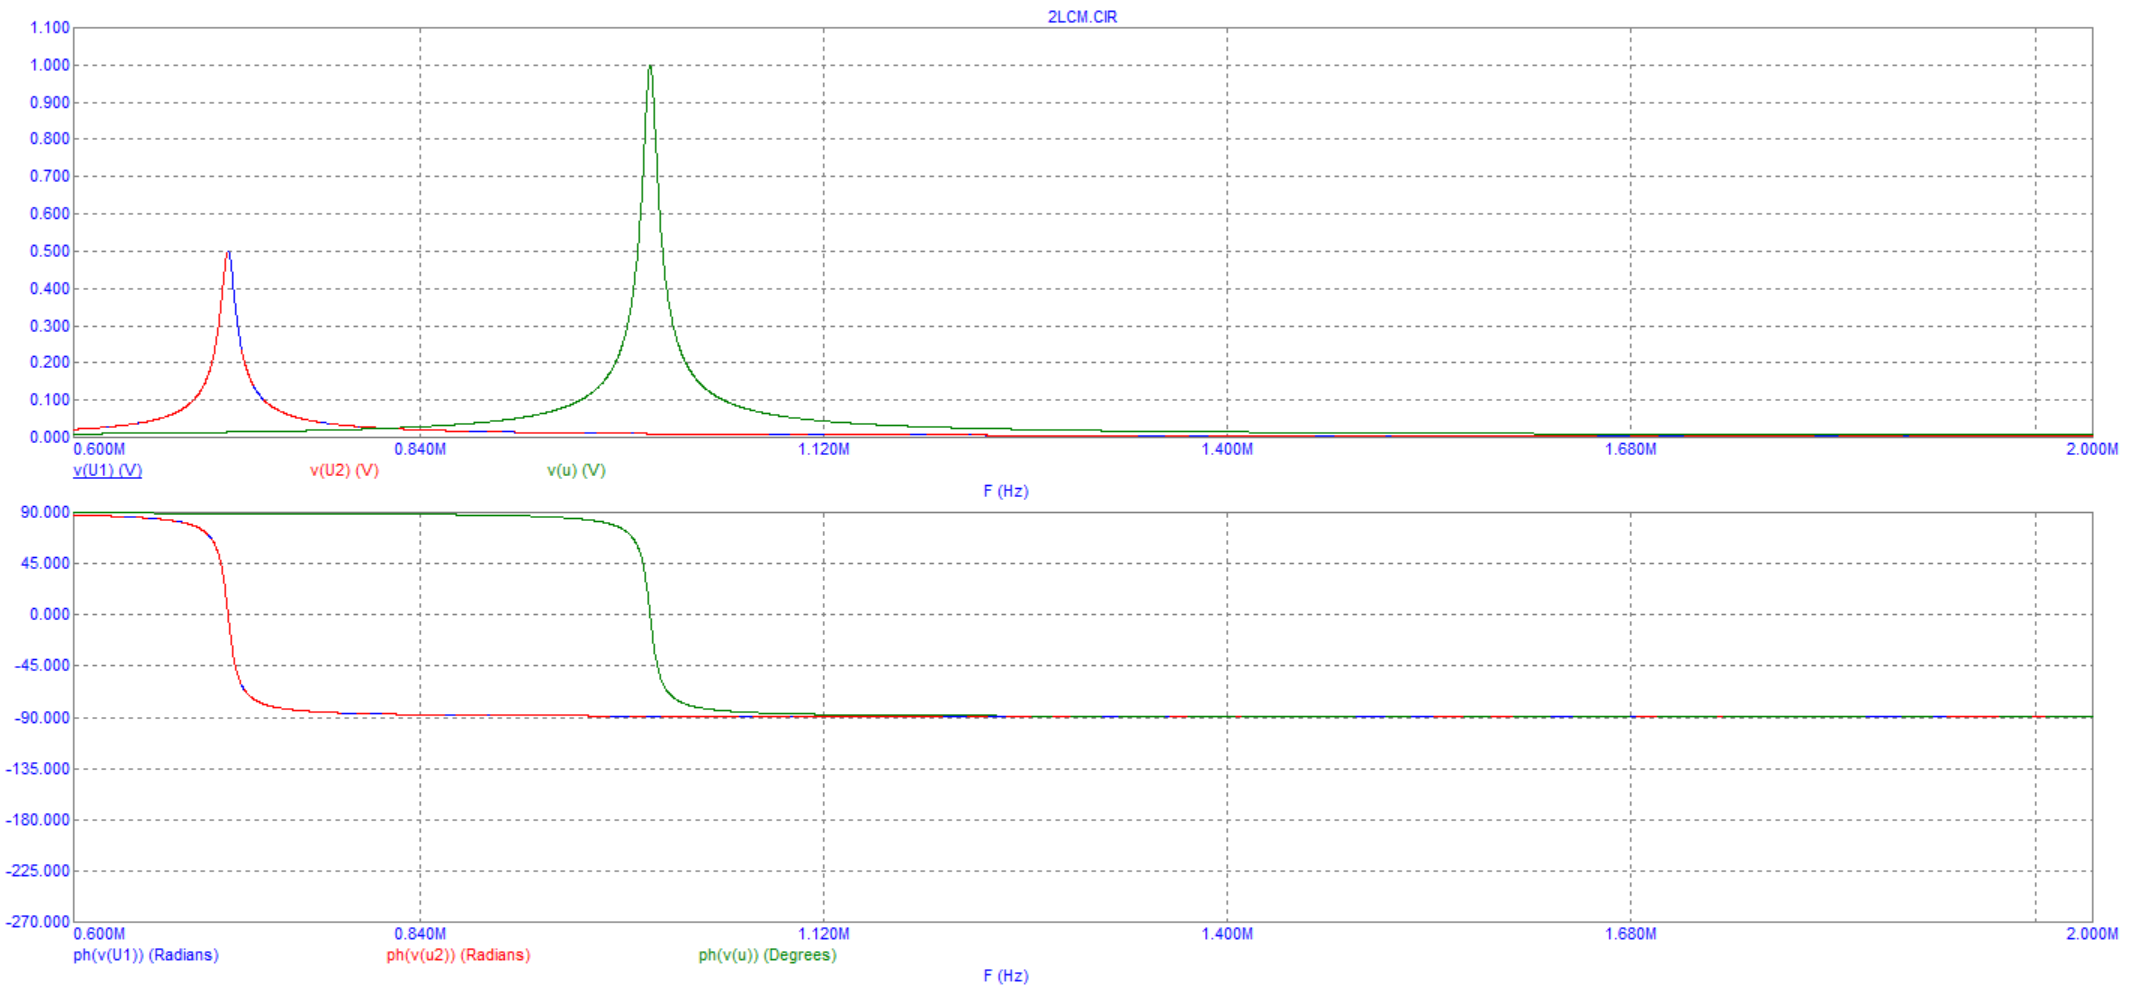
\includegraphics[scale = 0.4]{images/plot11_2.png}
\caption{$F \longrightarrow 100$}
\label{fig:Image1}
\end{figure}

\end{enumerate}

\newpage

\section{Система с емкостной связью}

\begin{enumerate}

\item Откроем модель 2LCC.CIR. 

\begin{figure}[h!]
\centering
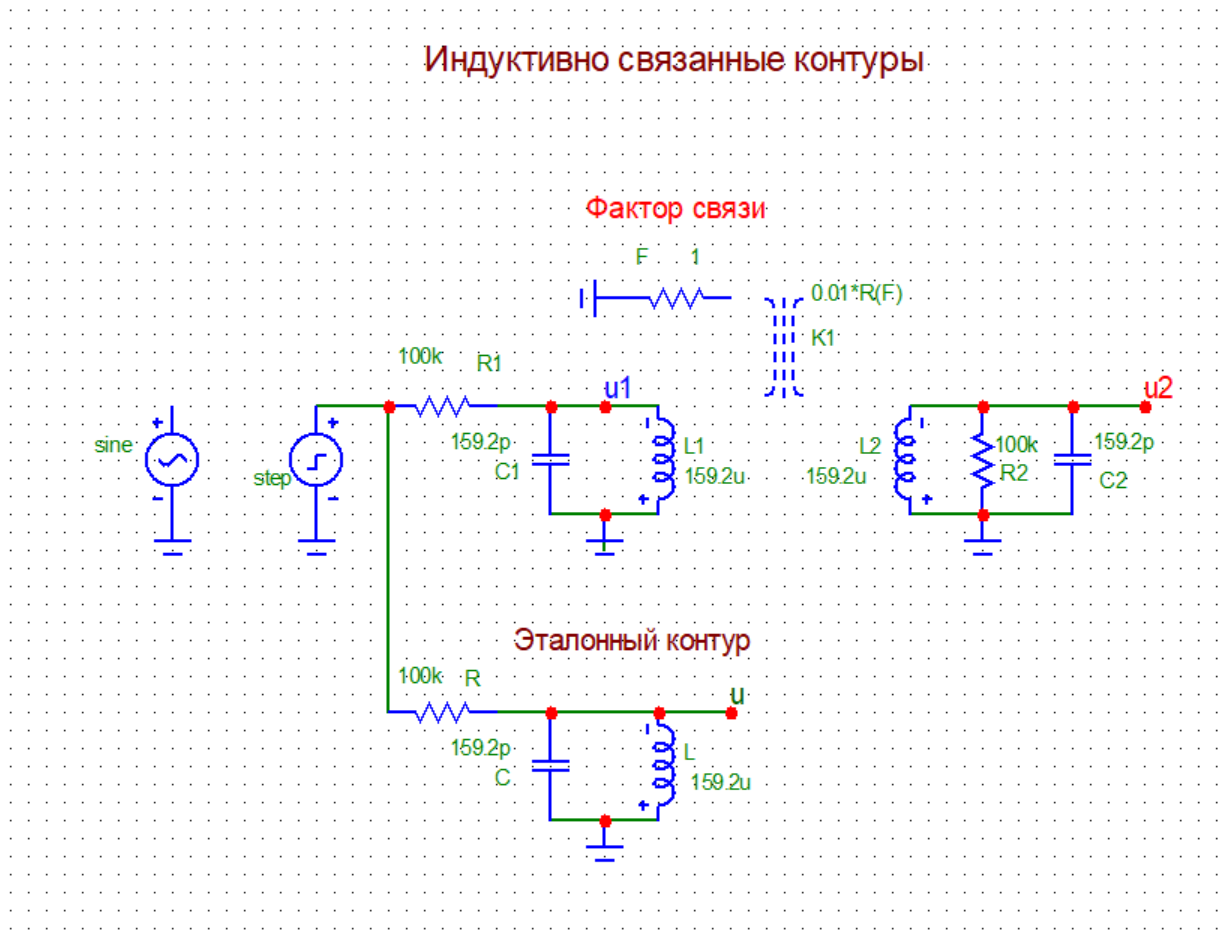
\includegraphics[scale = 0.7]{images/2LCM.png}
\label{fig:Image1}
\end{figure}

Проанализируем поведение частотных и фазовых характеристик при варьировании $F = [1,4|1]$. Соспоставим результаты наблюдений с картой полюсов/нулей на рис.11 в методичке.

\begin{figure}[h!]
\centering
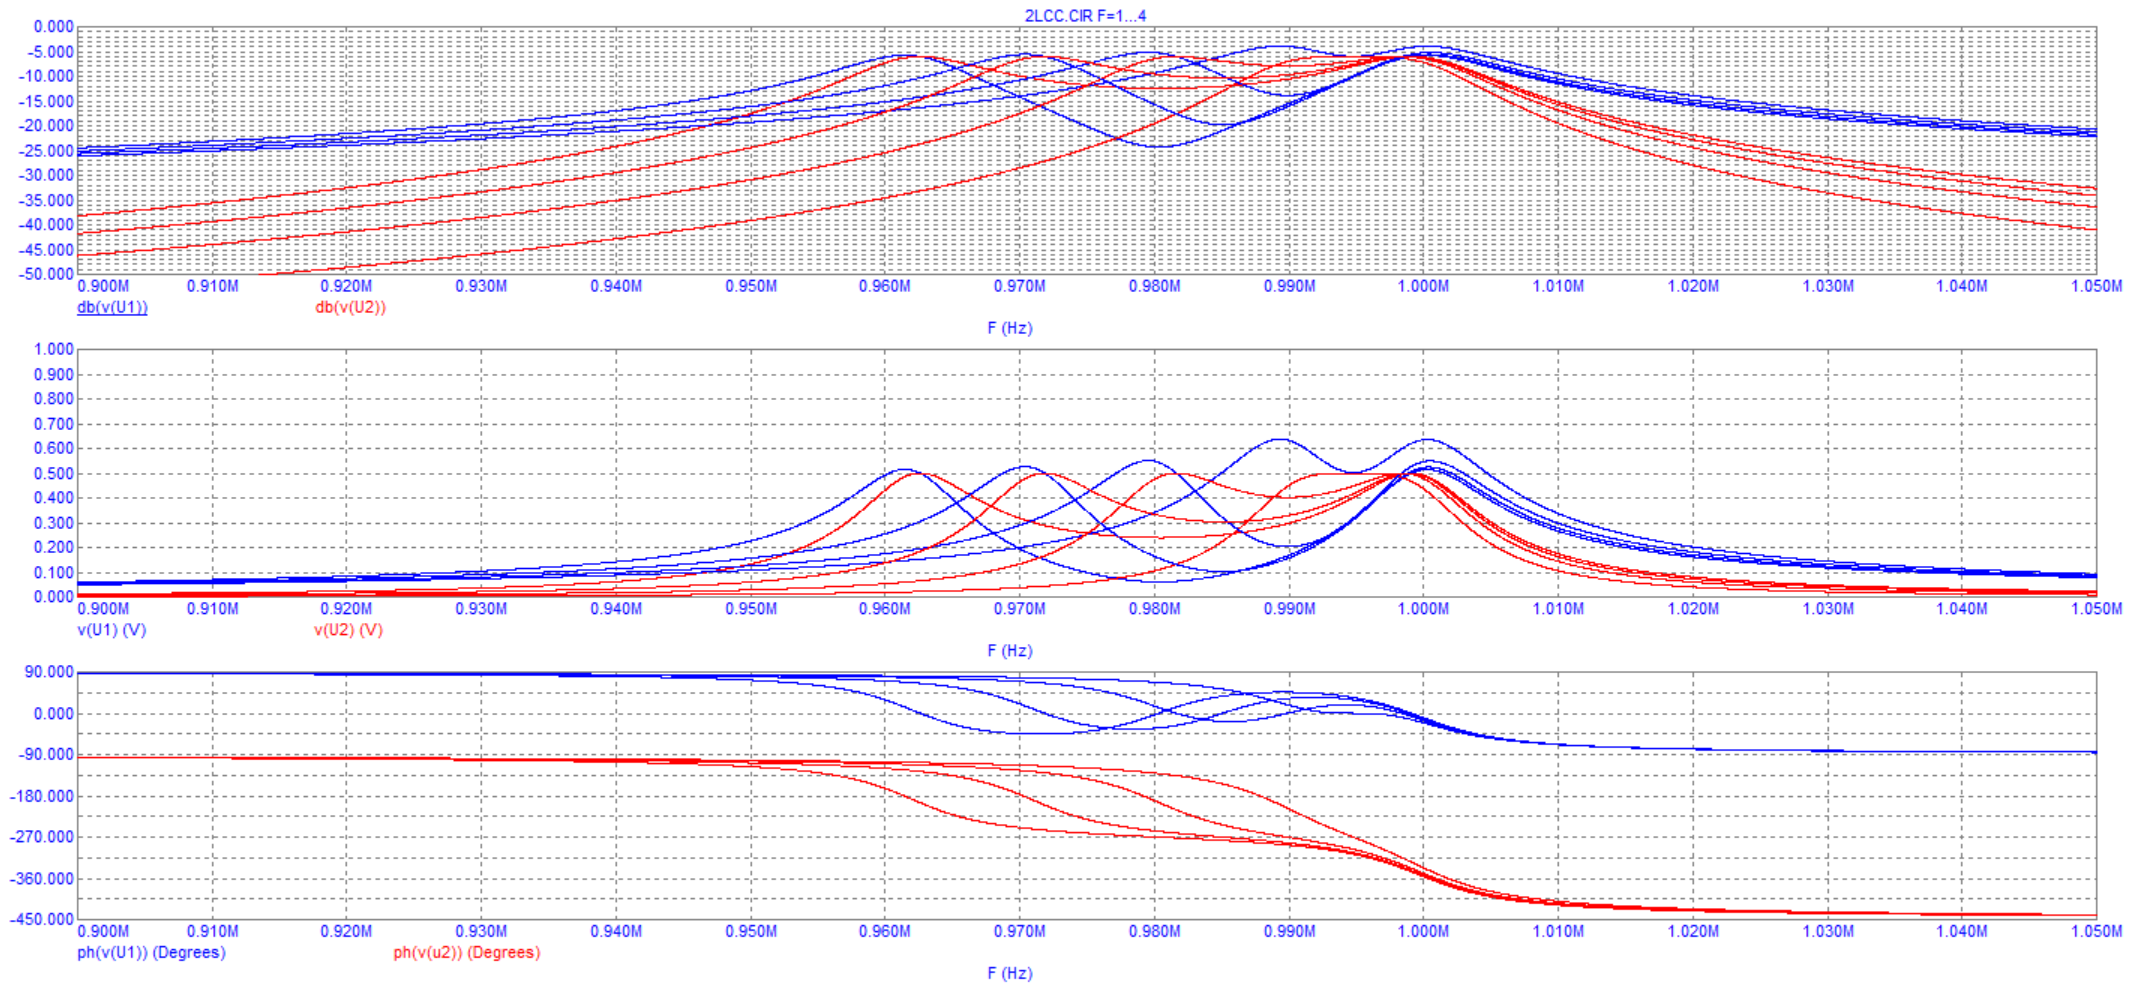
\includegraphics[scale = 0.4]{images/plot2-1_1.png}
\caption{$F = [1,4|1]$}
\label{fig:Image1}
\end{figure}

Измерим диапазоны изменения фазовых характеристик на первом и втором контурах.

На первом: от $90^{\circ}$ до $-90^{\circ}$.

На втором: от $-90^{\circ}$ до $-450^{\circ}$.

\vspace{0.5cm}

Измерим значения $F$, при которых:

a) возникает провал на первом контуре $F = 0.5$

b) провал на втором контуре $F = 1$

c) подъем на фазовой характеристике первого контура $F = 1$

\begin{figure}[h!]
\centering
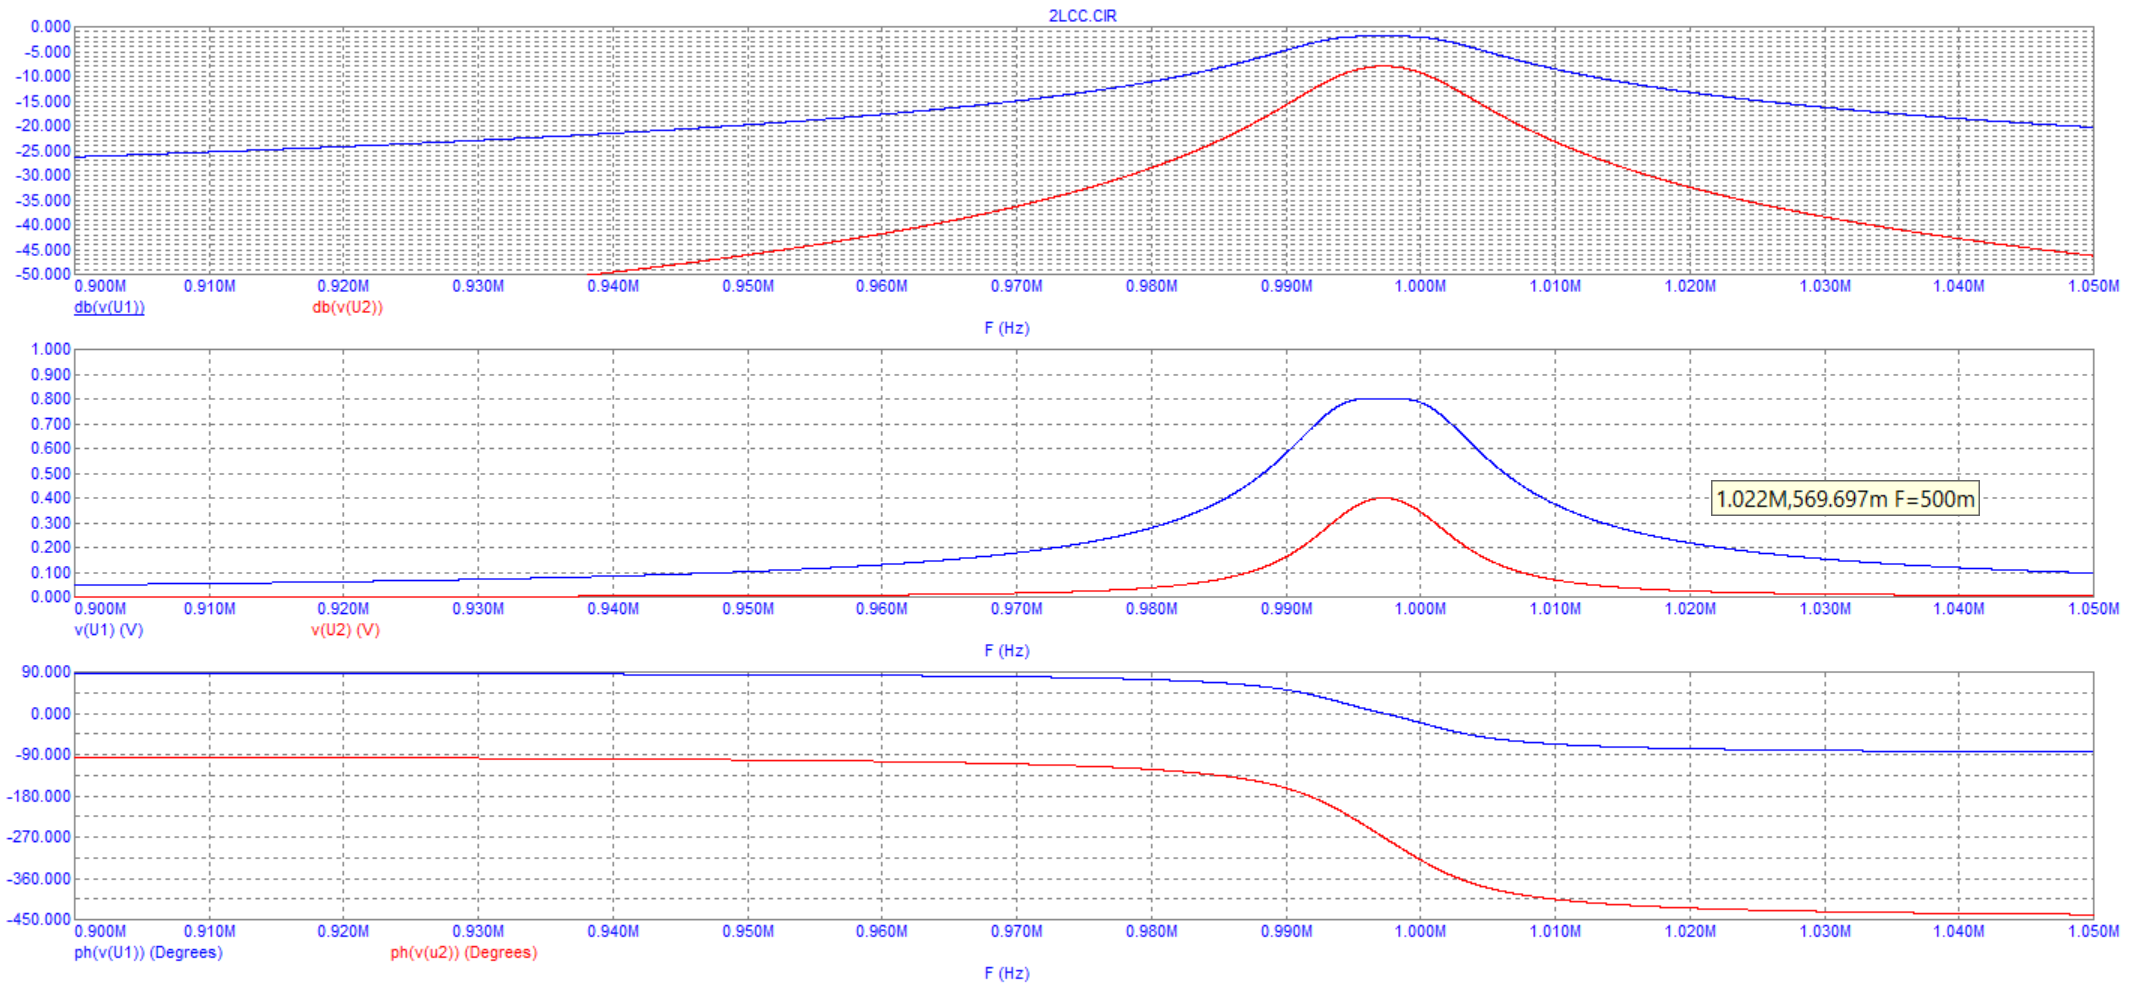
\includegraphics[scale = 0.4]{images/plot2-1_2.png}
\caption{$F = 0.5$}
\label{fig:Image1}
\end{figure}

Снимем зависимостьчастоты провала на втором контуре от $F = [2,4|1]$:

\begin{center}
\begin{tabular}{|c|c|c|c|}
\hline 
F & 2 & 3 & 4 \\ 
\hline 
$f_{\text{пров}}$, Гц & 990k & 985k & 980k \\ 
\hline 
\end{tabular} 
\end{center}

\newpage

\item Откроем график частотных характеристик в децибелах. Исследуем их изменение при варьировании $F = [1,4|1]$. Измерим уровни затухания при расстройках $\pm 50k$ (на декаду полосы контура). 

\begin{center}
\begin{tabular}{|c|c|c|}
\hline 
F & 1 контур, $\frac{dB}{\text{дек}}$ & 2 контур, $\frac{dB}{\text{дек}}$ \\ 
\hline 
1 & -20 & -39.7 \\ 
\hline 
2 & -19.5 & -34.7 \\ 
\hline 
3 & -19 & -27.6 \\ 
\hline 
4 & -18 & -26 \\ 
\hline 
\end{tabular} 
\end{center}

Перейдем на частотный диапазон [$10Meg, 100k$] и измерим уровни затухания при расстройках на декаду $f_0$:

\begin{center}
\begin{tabular}{|c|c|c|c|}
\hline 
F & 1 контур, $\frac{dB}{\text{дек}}$ & 2 контур (100k), $\frac{dB}{\text{дек}}$ & 2 контур (10Meg), $\frac{dB}{\text{дек}}$ \\ 
\hline 
1 & -60 & -141 & -102 \\ 
\hline 
2 & -60 & -132 & -96 \\ 
\hline 
3 & -60 & -129 & -92 \\ 
\hline 
4 & -60 & -126 & -88 \\ 
\hline 
\end{tabular} 
\end{center}

\newpage

\item Изучим переходные характеристики при значениях $F = 0.1; 2; 3; 4.$ Убедимся в их сходстве с характеристиками системы с индуктивной связью.

\begin{figure}[h!]
\centering
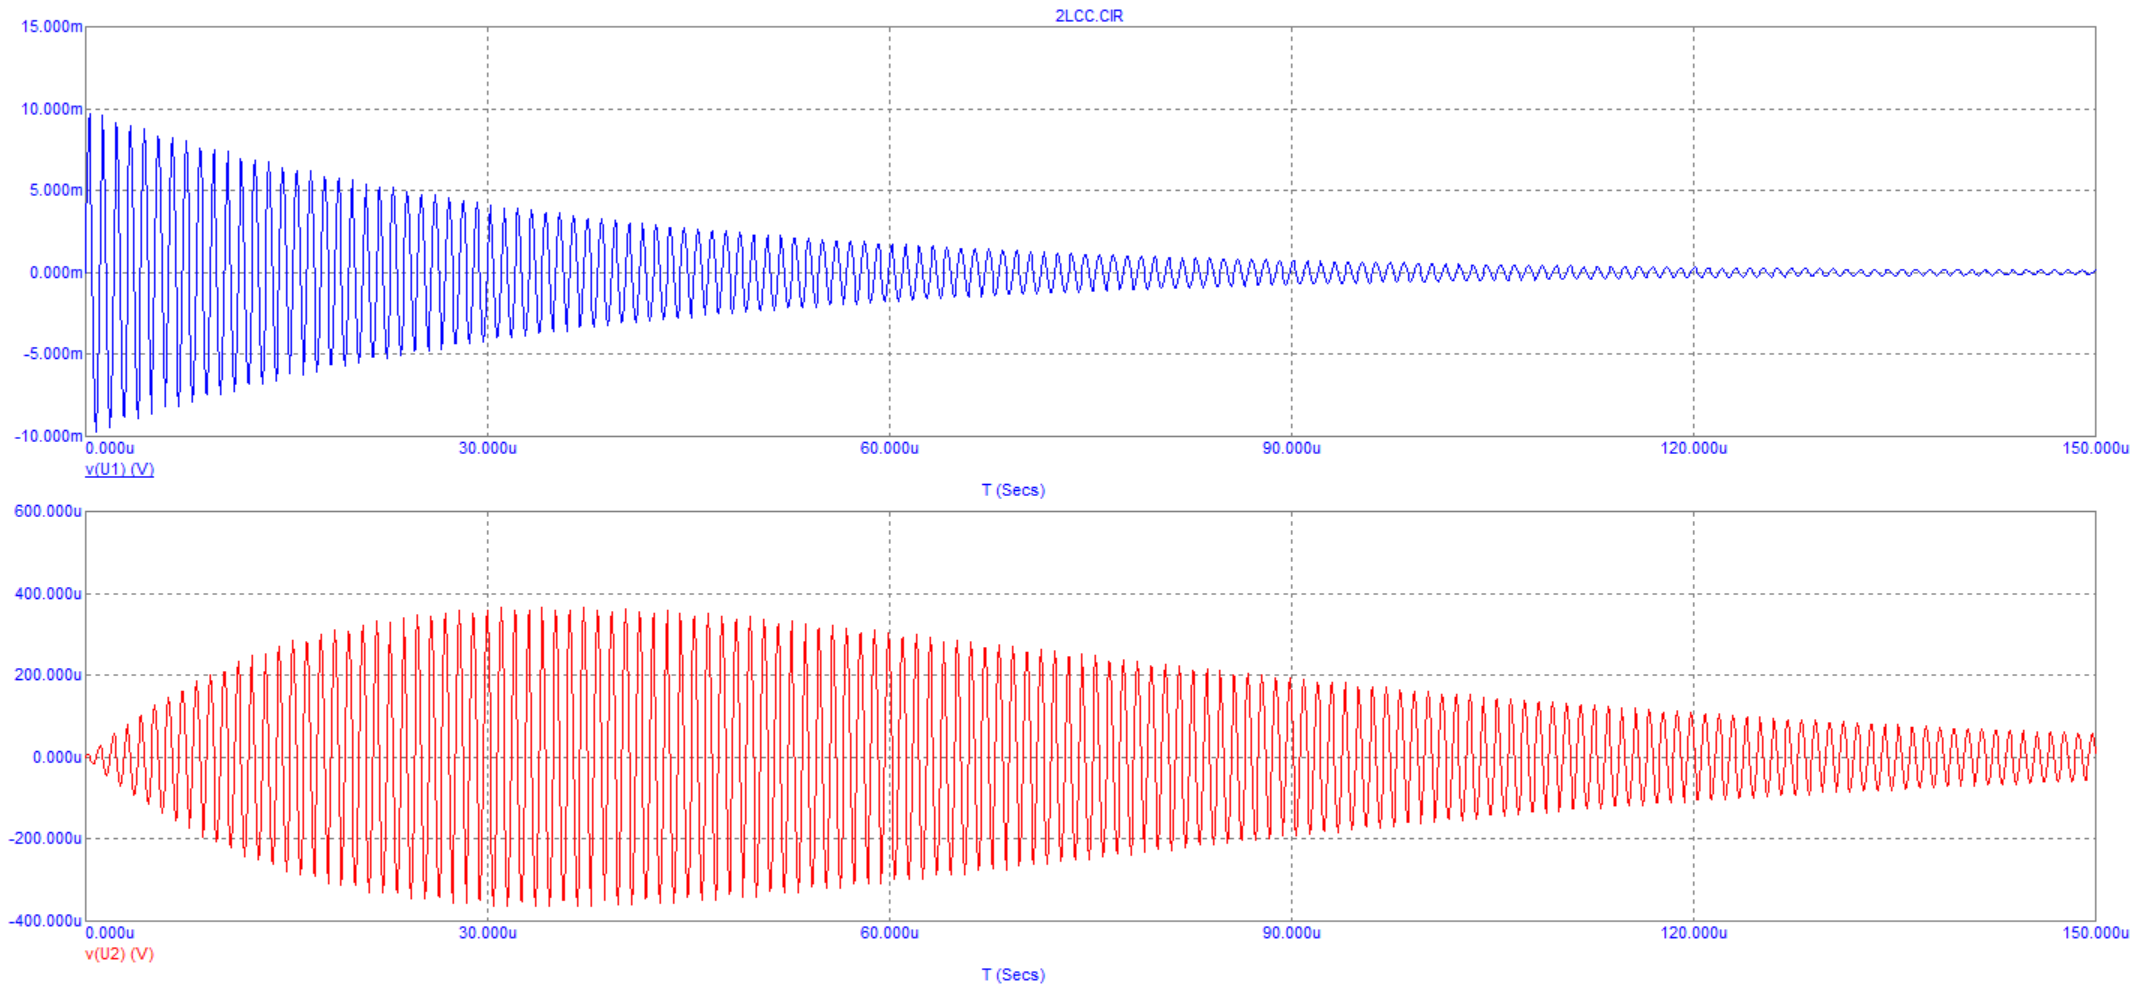
\includegraphics[scale = 0.4]{images/plot2-1_3.png}
\caption{$F = 0.1$}
\label{fig:Image1}
\end{figure}

\begin{figure}[h!]
\centering
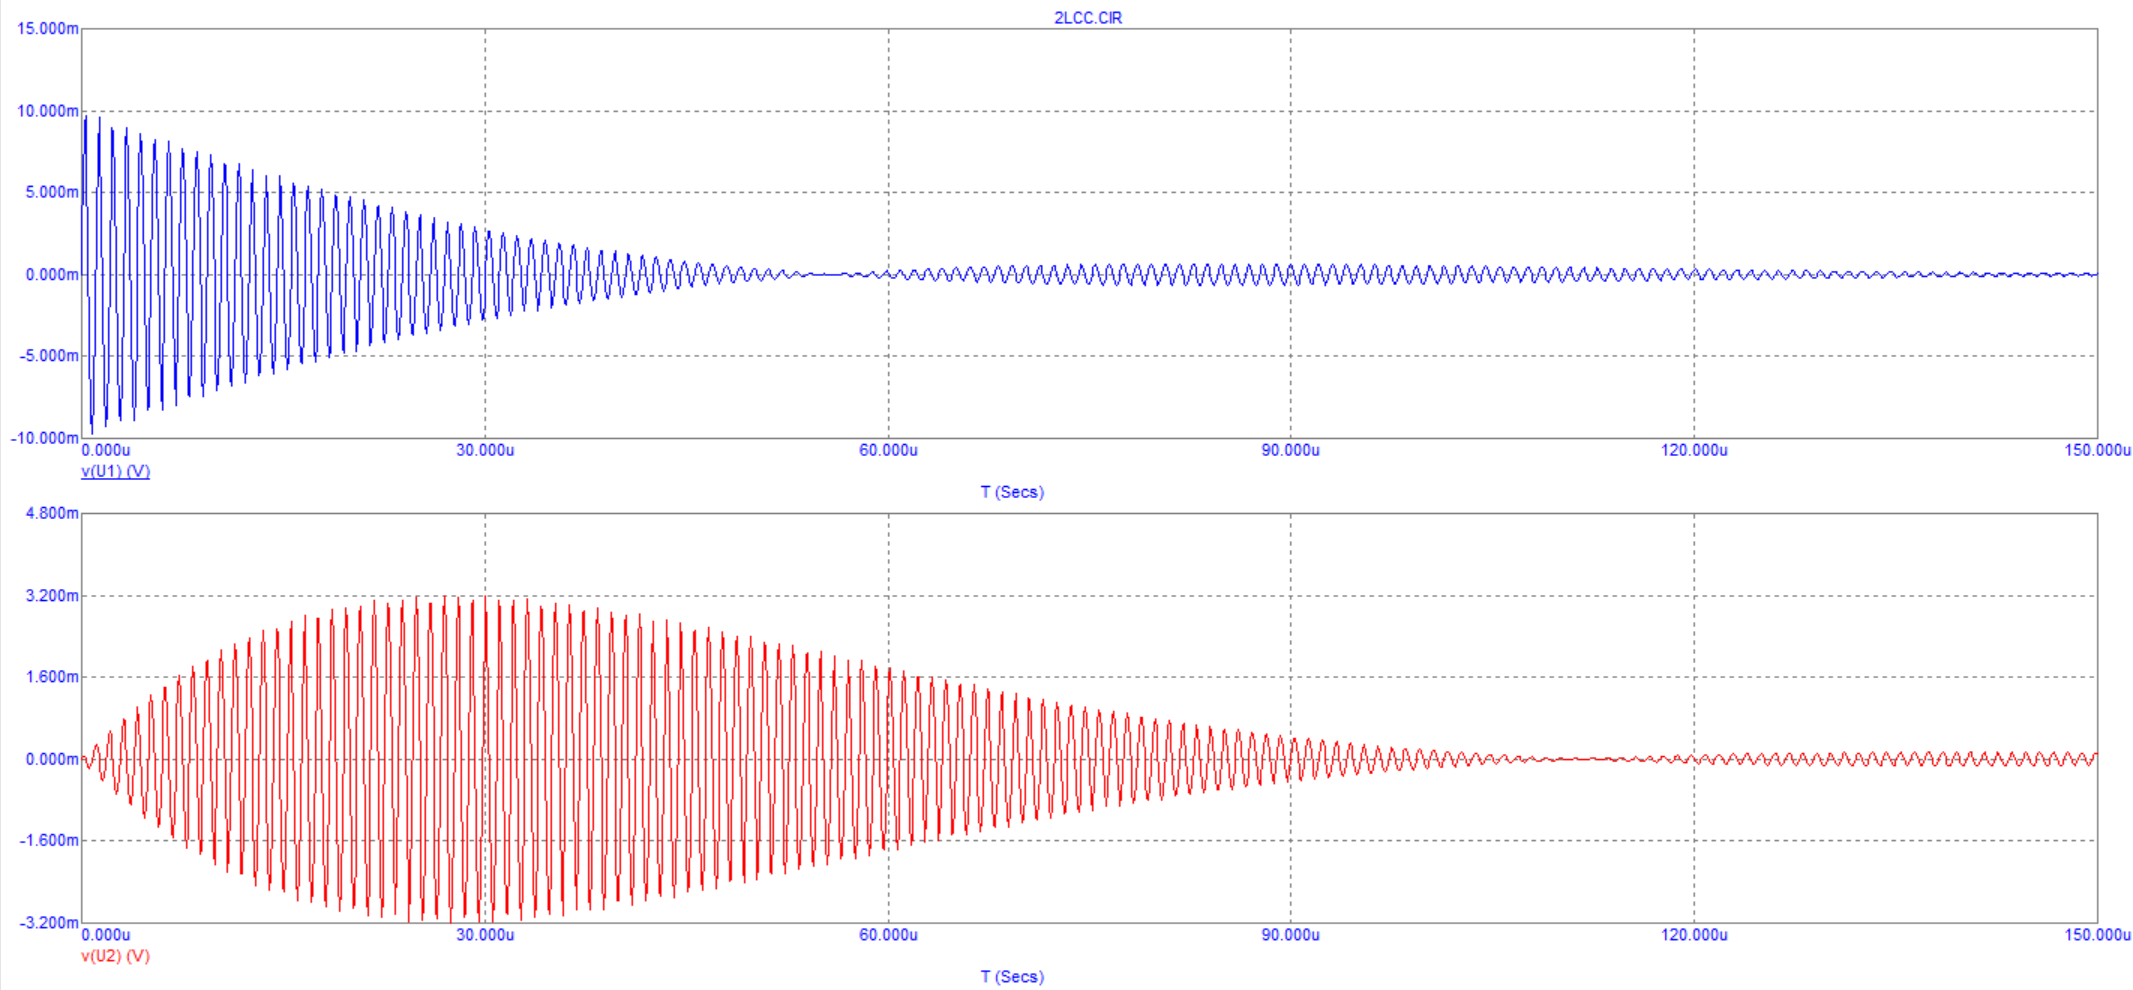
\includegraphics[scale = 0.4]{images/plot2-2_3.png}
\caption{$F = 1$}
\label{fig:Image1}
\end{figure}

\begin{figure}[h!]
\centering
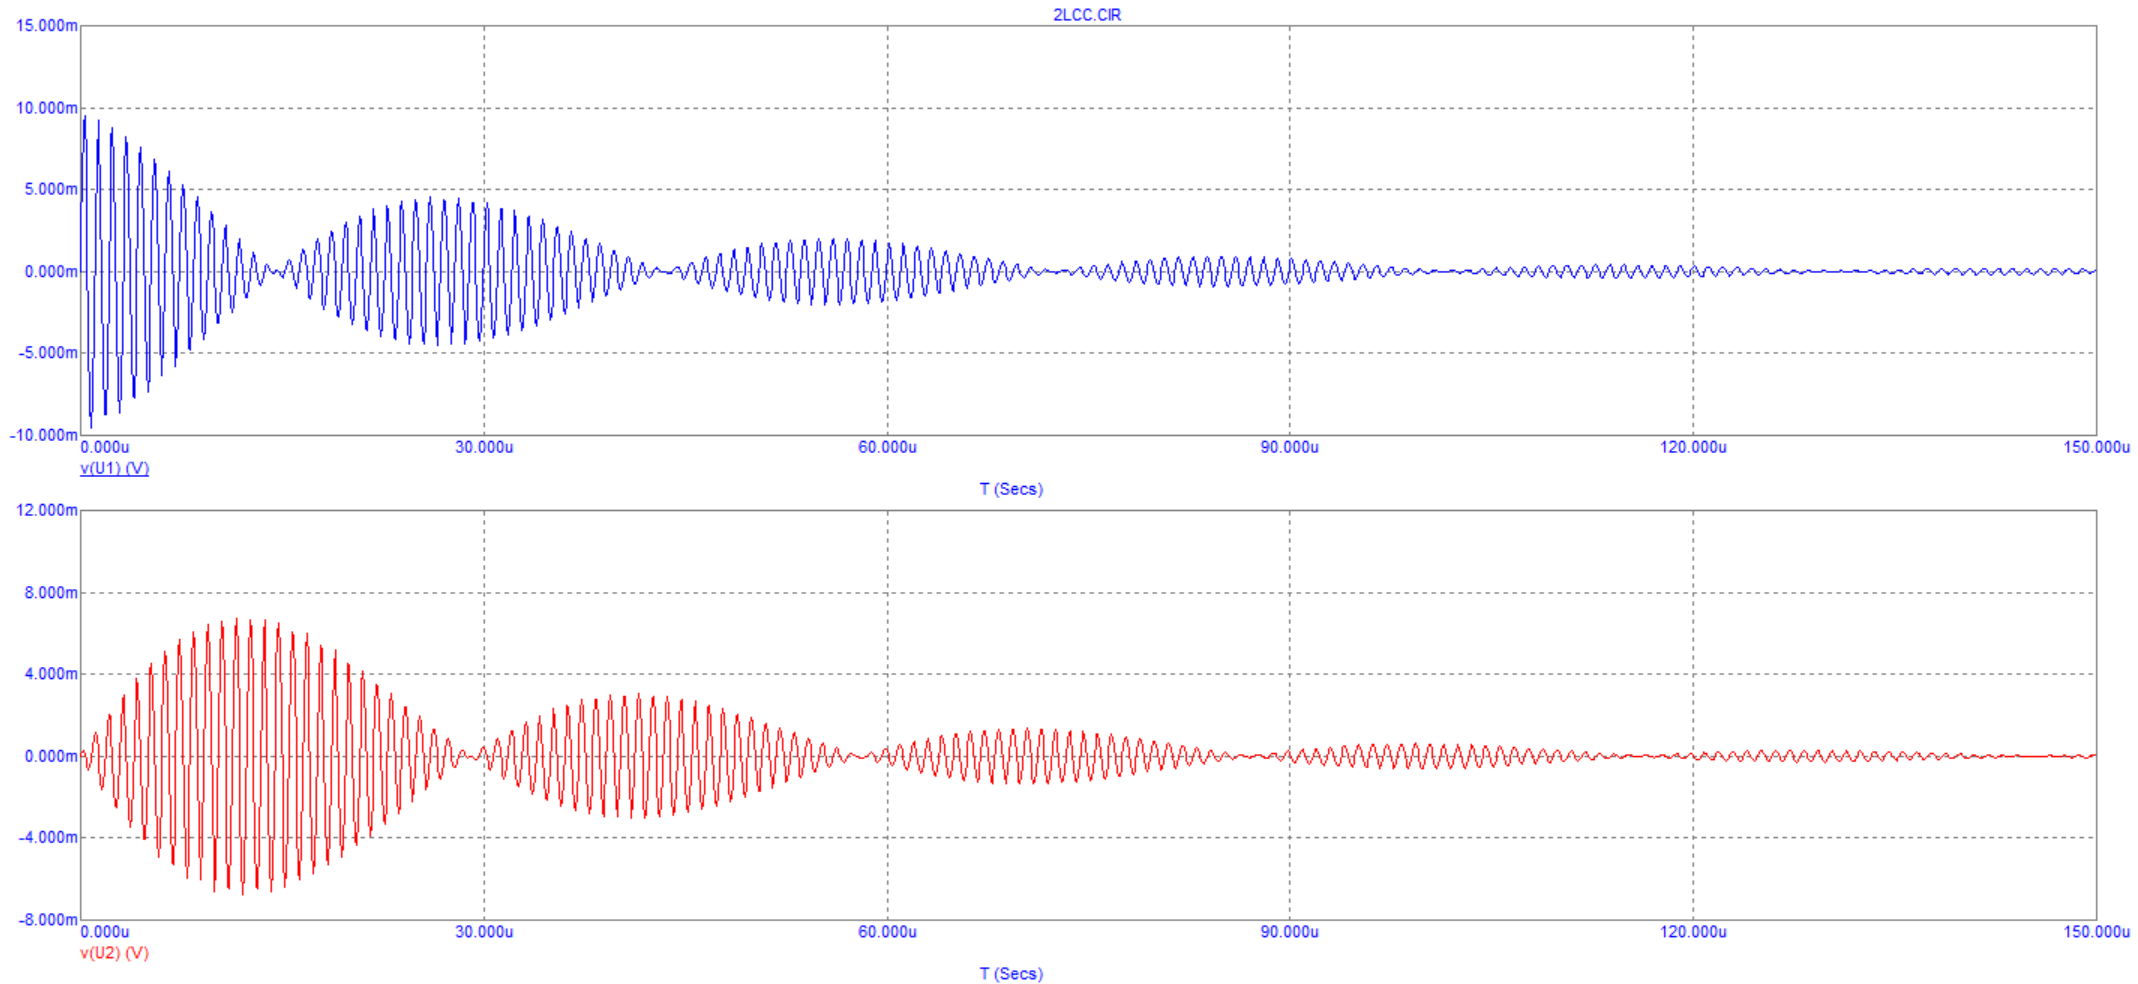
\includegraphics[scale = 0.4]{images/plot2-3_3.png}
\caption{$F = 4$}
\label{fig:Image1}
\end{figure}

\end{enumerate}

\end{document}